\chapter{Simulation and Results}
\label{chap:simulationandresults}

In this chapter, different scenarios for the simulation and their results will be exposed and commented. To make it easier to understand, and as 
previously this two cases were also separated, first just the Sync Phase will be analyzed and then the whole protocol together.

In all the scenarios, simulations are independent among them and at least 100 repetitions are going to be done, this way the confidence intervals
shown in all figures could be calculated like in (\ref{mat:confidenceintervals}).

\begin{equation}
  x-\frac{\sigma}{\sqrt{n}}\cdot t_{\frac{\alpha}{2}} < \mu < x+\frac{\sigma}{\sqrt{n}}\cdot t_{\frac{\alpha}{2}}
  \label{mat:confidenceintervals}
\end{equation}

Where x is the value to check, $\sigma$ is the standard deviation of the measurements, $\mu$ is the average value, n is the number of repetitions done and 
$t_{\frac{\alpha}{2}}$ is a constant of 1.96 for a confidence interval of 95\%.

\section{Sync Phase simulation and analysis}

The aim of this section is to compare slotted transmission and random transmission during Sync Phase. This two approaches were already commented 
during Chapter \ref{chap:protocoldesign}: \nameref{chap:protocoldesign}.

As random transmission case is more difficult and chaotic as the slotted one, this will be studied separately first, leaving the slotted case to 
be studied together with the comparison and finishing with a study of the number of slots depending on the \acp{AN} density.

\subsection{Random Transmission}

To study this case, scenarios in Figure \ref{fig:hiddenvsnohidden} were simulated. In a) can be seen that all nodes can detect all node transmissions,
avoiding so Hidden Terminal Problem. In b), \acp{AN} can detect only some of the \ac{AN} transmissions and the \ac{MN} can detect all of them, this way
\acp{AN} are going to start transmitting when probably another \ac{AN} will be doing so, provoking a collision at the \ac{MN}. The number of \acp{AN}
is 6 in both cases and the number of \acp{MN} is 1.

\begin{figure}[ht]
 \begin{center}
  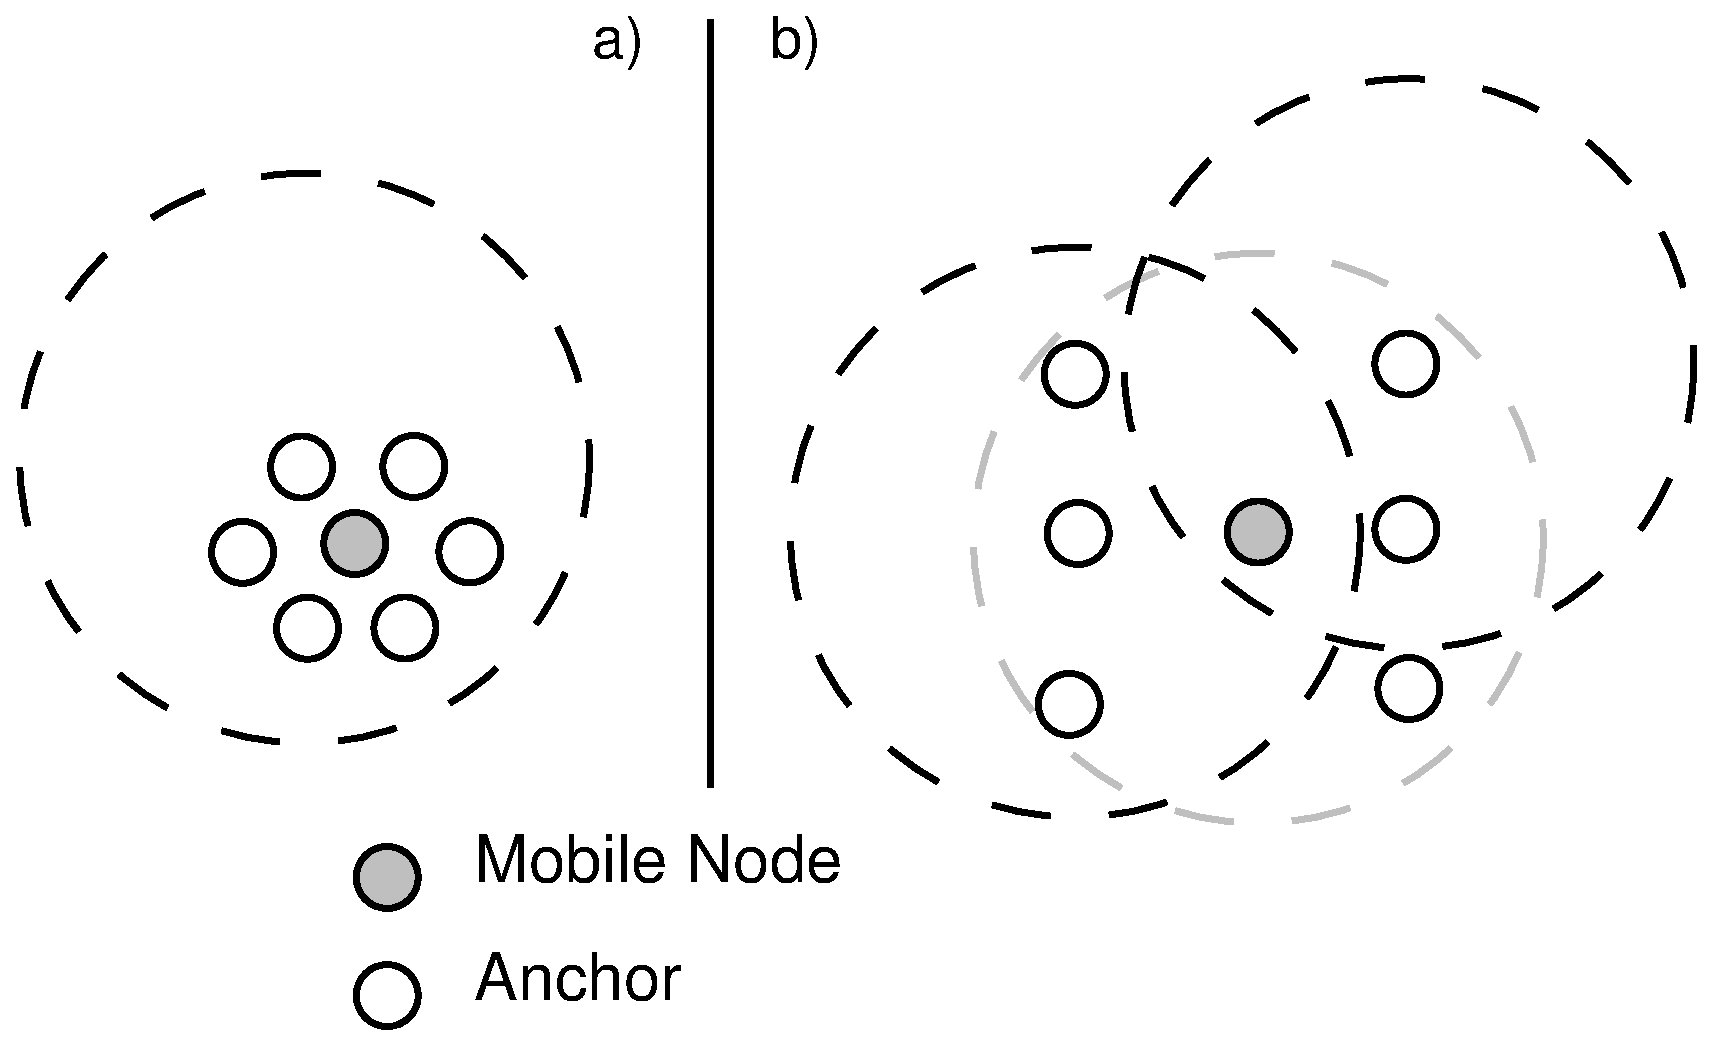
\includegraphics[width=0.5\textwidth]{hiddenvsnohidden.eps}
 \end{center}
 \caption{Scenarios avoiding (a) and forcing (b) Hidden Terminal Problem}
 \label{fig:hiddenvsnohidden}
\end{figure}

All errors caused by noise and random errors due to the channel, were disabled during this simulation. This is so, to have only simultaneous \acp{CCA} 
problem and Hidden Terminal Problem. With this situation, it can be assured that if a packet is received incorrectly in the \ac{MN}, the reason would 
be one of this two problems.

As is was commented in Chapter \ref{chap:protocoldesign}: \nameref{chap:protocoldesign}, in order to avoid an unknown random time during active 
synchronization, \ac{CSMA/CA} must be disabled. If this is done, all \acp{AN} will transmit at the same time generating lots of collisions. To solve this
a random time is added by Application Layer before the packet is transmitted. This random time value, will be between 0 and a maximum number. In this
section, this maximum number goes from 1 to 30 originating 30 different simulations. This value will be the X axis in all Figures. 

In order to reduce the dispersion caused by random numbers, each simulation will be done 1000 times.

\begin{figure}[ht]
 \begin{center}
  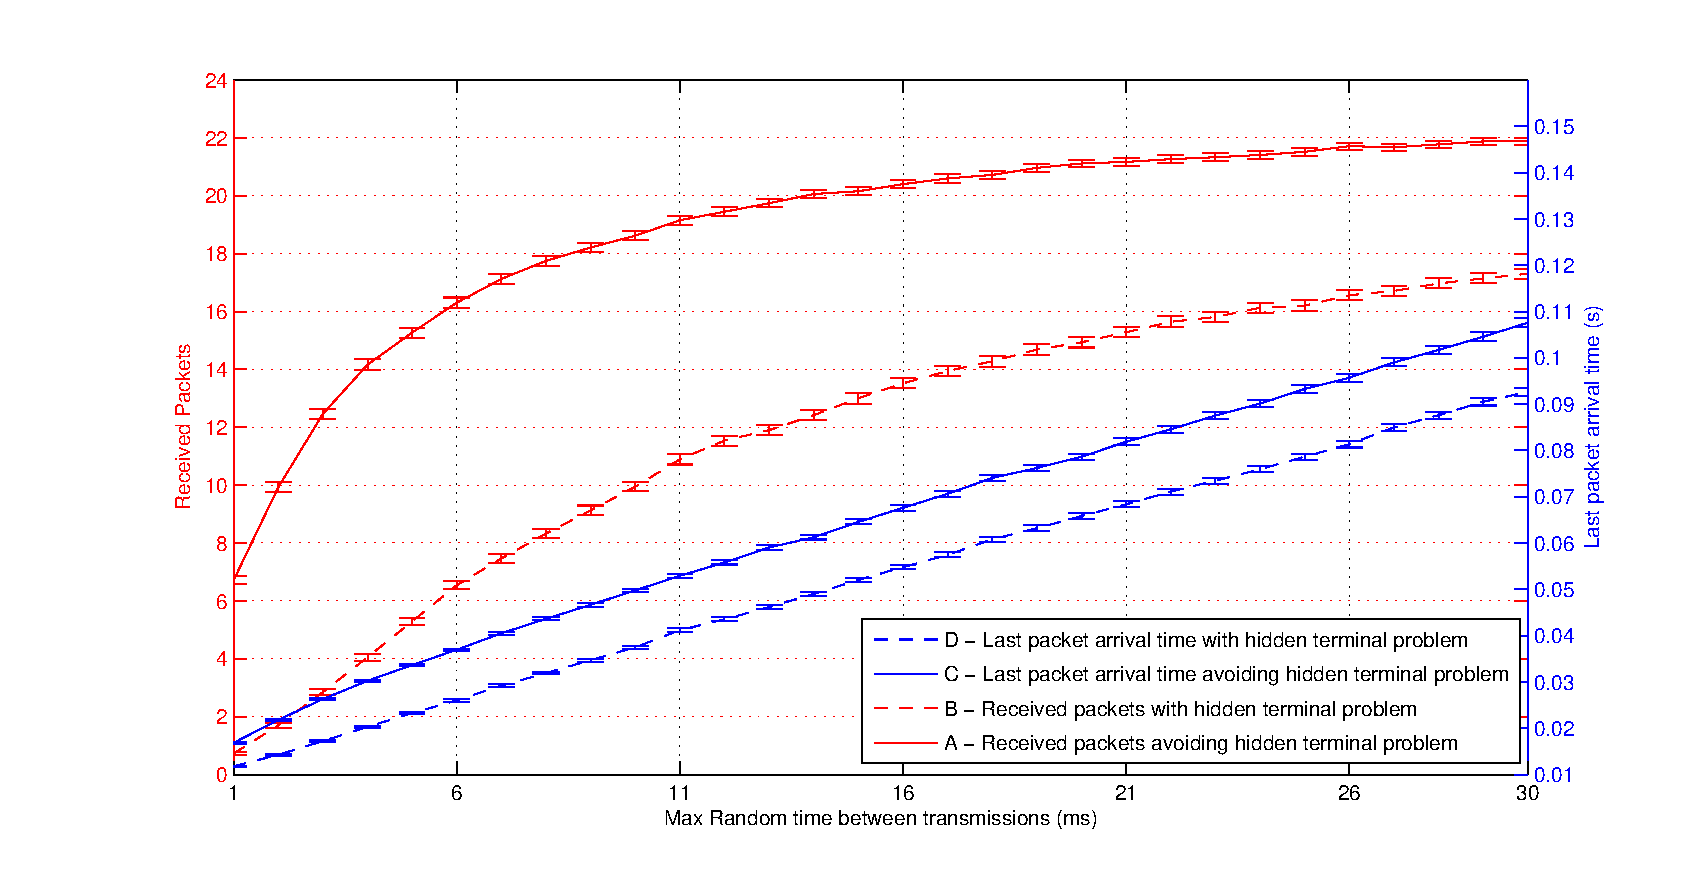
\includegraphics[width=1\textwidth]{receivedPacketsAndLastPacketArrival.eps}
 \end{center}
 \caption{Received packets in \ac{MN} and last packet arrival time}
 \label{fig:receivedPacketsAndLastPacketArrival}
\end{figure}


First simulation, gives as result \textbf{Figure \ref{fig:receivedPacketsAndLastPacketArrival}}. Here can be seen the total received packets in the 
\ac{MN} and the time when the last packet arrived in function of the maximum inter packet transmission time.

Both received packets lines (A and B) have a rising trajectory and both tend to 24 in the infinite. This 24 packets are the total number of 
packets sent to the network, sending each \ac{AN} four. It can be seen that, as in the case without Hidden Terminal Problem (A) the number of collisions
is smaller, the number of received packets in the \ac{MN} is much bigger than in the Hidden Terminal Problem case.

This Figure shows also the average arrival time from the last arrived packet in the \ac{MN}. This is not the 24$^{th}$ sent packet, as this could 
possibly collide with another. As the number of arrived packets in the case avoiding Hidden Terminal Problem is bigger, the last packet takes more time 
to arrive to the \ac{MN}. This can be seen in the Figure as C line values are always bigger than D line ones.

\begin{figure}[ht]
 \begin{center}
  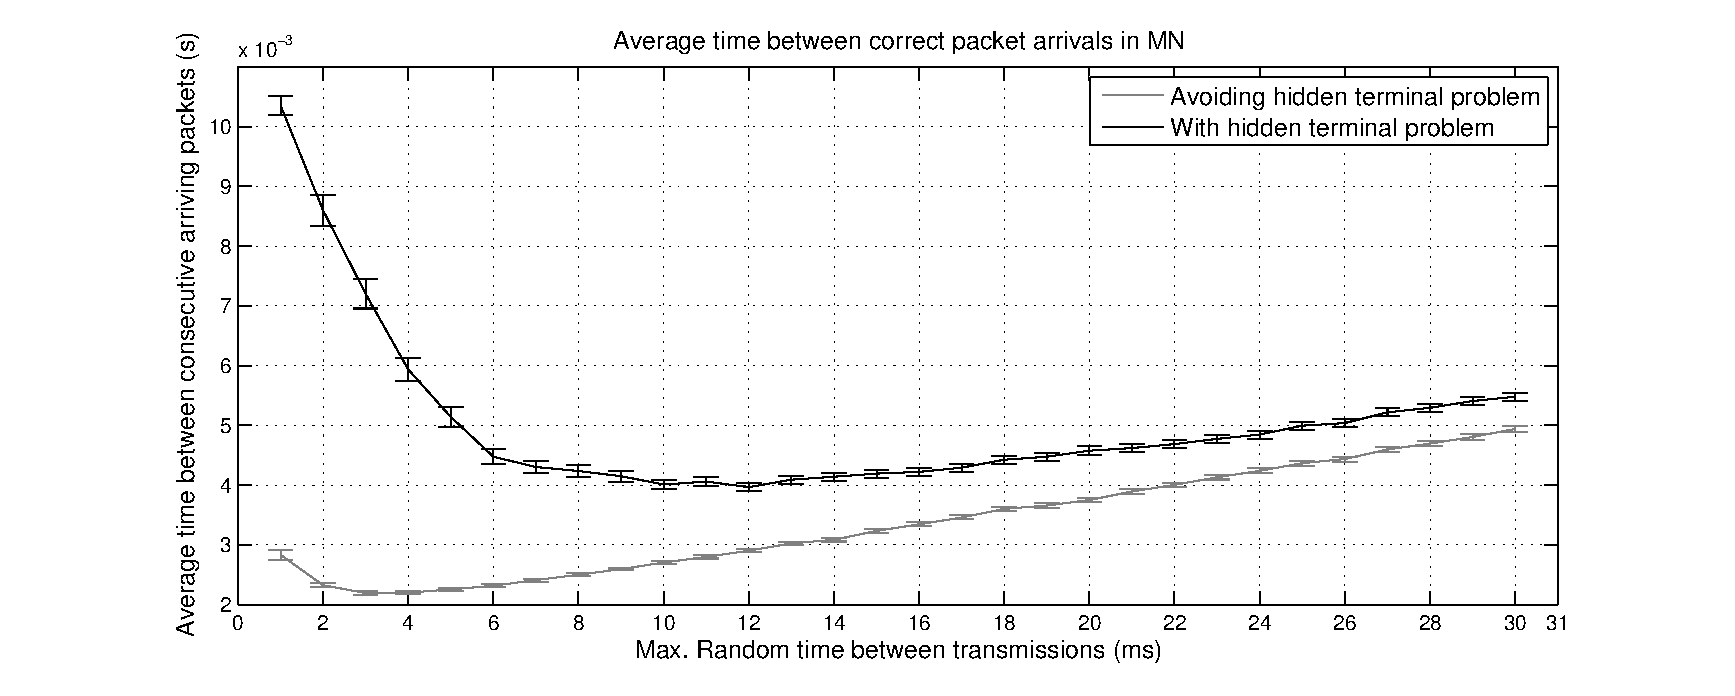
\includegraphics[width=1\textwidth]{averageTimeBetweenArrivals.eps}
 \end{center}
 \caption{Average time between arrivals in the \ac{MN}}
 \label{fig:averageTimeBetweenArrivals}
\end{figure}

\textbf{Figure \ref{fig:averageTimeBetweenArrivals}} shows the average times between packet arrivals in function of the maximum inter packet 
transmission time. This time does not represent the arrival time between two packets from the same \ac{AN}, but from any \ac{AN}. It is seen how
for the case with Hidden Terminal Problem, the time between consecutive arrived packets is much bigger than for the case without Hidden Terminal Problem,
consequently the number of collisions is also bigger, needing the \ac{MN} to wait more time until it gets another valid packet.

It is logic to think, that the bigger the time between transmissions, the bigger the time inter arrived packets. But, why in both cases, with or 
without Hidden Terminal Problem, for low values in X axis, the Y values start high and decrease until a certain moment where they start to grow again? 
This is because at the beginning, when the time between transmissions is low, the number of collisions is high as all \acp{AN} are trying to send their
packets almost at the same time. As the X value becomes bigger, the number of collisions gets reduced and thus the inter packet arrival time. But from 
the moment where the curves make their minimum, the influence of the time between transmissions becomes important, and makes the curves go up again.

\begin{figure}[ht]
 \begin{center}
  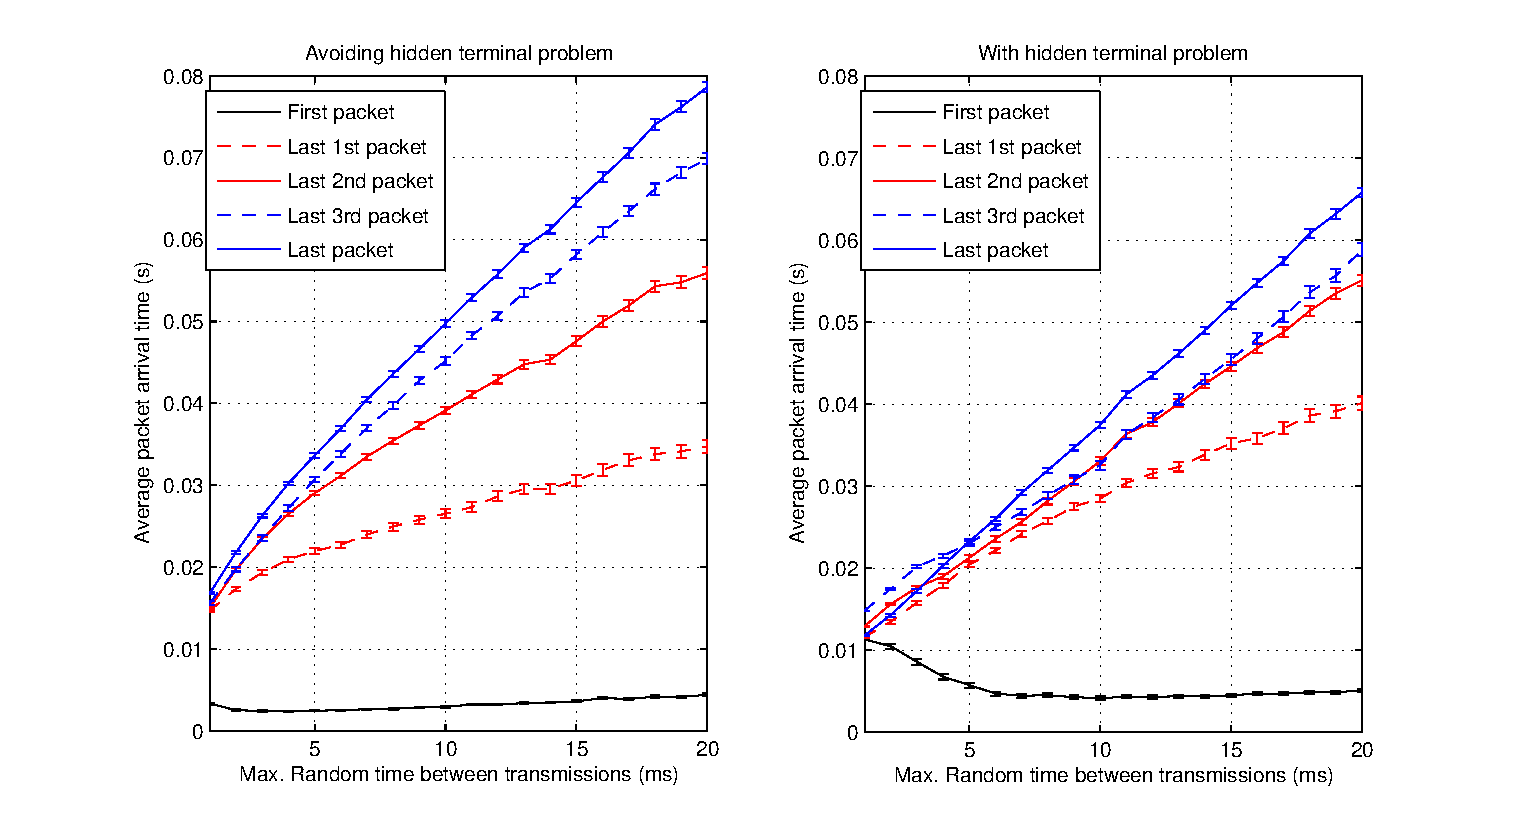
\includegraphics[width=1\textwidth]{averageDifferentTimes.eps}
 \end{center}
 \caption{Packet arrival average times}
 \label{fig:averageDifferentTimes}
\end{figure}

\textbf{Figure \ref{fig:averageDifferentTimes}} shows the average arrival time in the \ac{MN} of the first packet, the last first packet, the last
second packet, the last third packet and the last packet coming from any of the \acp{AN}.

It is easy to see that arrival time of the first packet should be smaller than the arrival time of the last first packet, this should be smaller than
 the arrival time of the last second packet, this should be smaller than last third and this smaller than the last. But if the case with Hidden 
Terminal Problem is observed, it can be found that when time between transmissions is small, last second and last third received packets arrive later 
that last received packet. How is this possible? This happens because due to the big number of collisions many times only first packets arrive or many of 
them arrive after the last second or third packets. When conditions are better (higher time between transmitted packets or no Hidden Terminal Problem) 
this does not happen because many more second or third packets are delivered and thus they will be the last packets.

It is also interesting how unlike the right figure, for the case without Hidden Terminal Problem, the arrival time of the first packet and the arrival 
time of the last first packet are quite separated. This is because in this case the collision number is much smaller, and as it was seen in Figure 
\ref{fig:receivedPacketsAndLastPacketArrival}, the \ac{MN} receives much more first packets from the \acp{AN}.

As comparison between the two cases, it can be seen that for the case without Hidden Terminal Problem, the arrival times are bigger, this is again because
the \ac{MN} receives in this case much more packets due to a lower number of collisions, making the last packets arrive later. This lower number of 
collisions makes also that the arrival time of the first packet is smaller than for the case with Hidden Terminal Problem.

\begin{figure}[ht]
 \begin{center}
  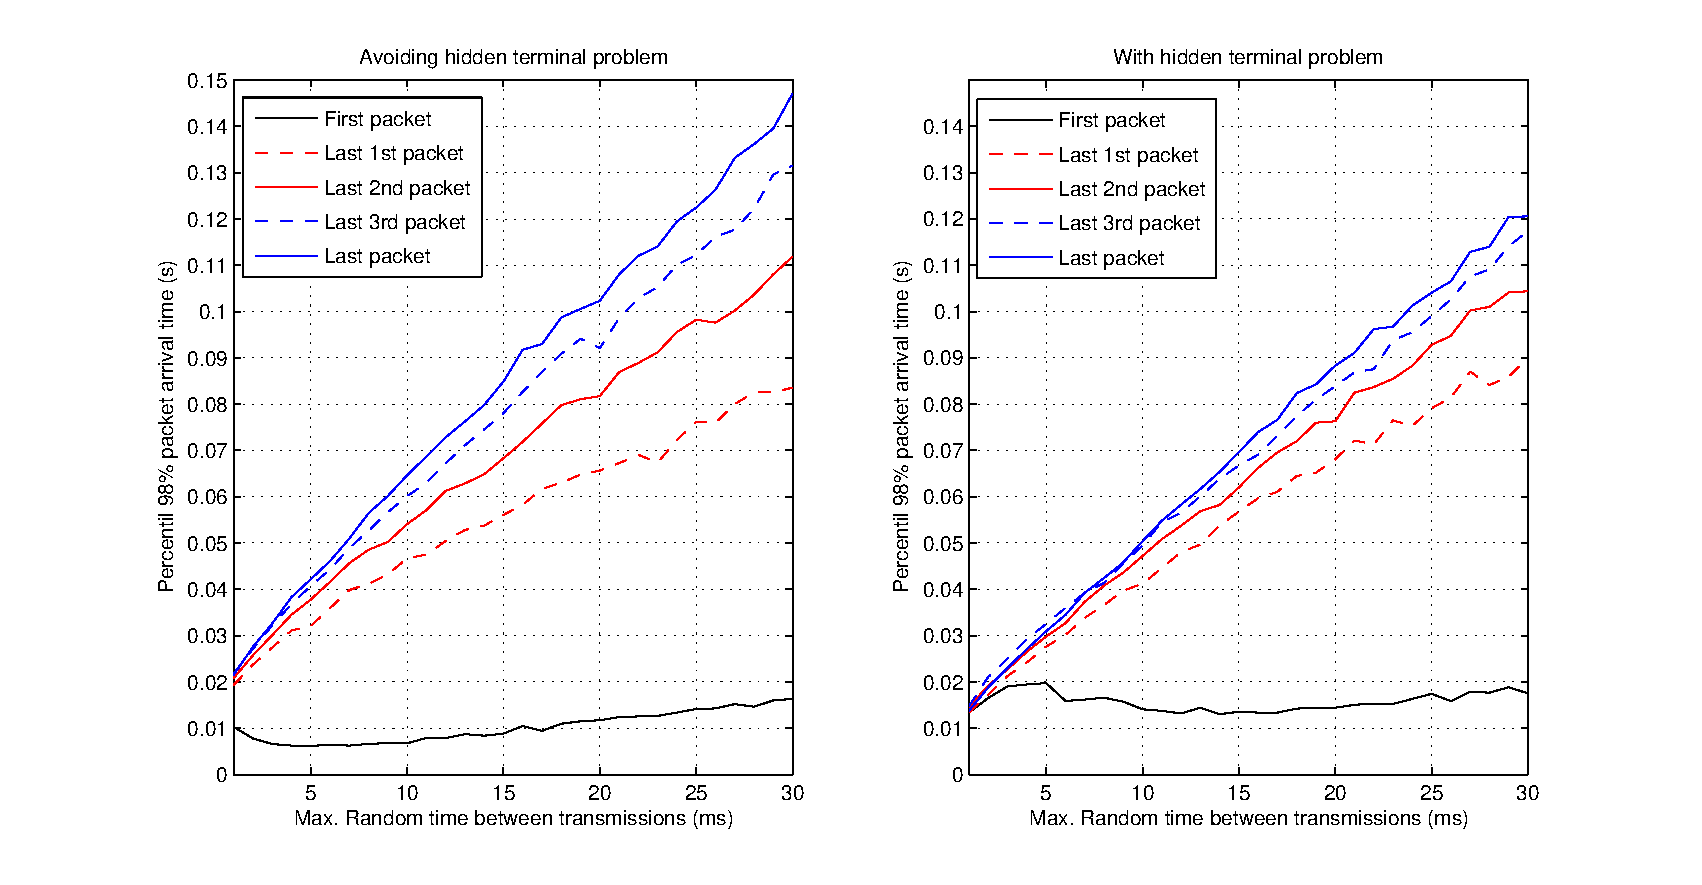
\includegraphics[width=1\textwidth]{percentil98differentTimes.eps}
 \end{center}
 \caption{Percentil 98 of packet arrival times}
 \label{fig:percentil98differentTimes}
\end{figure}

\textbf{Figure \ref{fig:percentil98differentTimes}} does not represent an average but a percentil 98, this means that if this times are taken as 
reference, in 98\% of the situations, the times are going to be under this values. This is thus a good way to get an acceptable top limit.

The analysis from this graphic is the same as the previous one with the only peculiarity that all times in Y axis are bigger, this is so because
this graphic represents the worst cases, not the average. For the same reason, in the case with Hidden Terminal Problem when the times between
transmissions are small, the first arrived packet time is bigger and behaves different as in Figure \ref{fig:averageDifferentTimes}.

\subsection{Slotted vs. Random Transmission}

The aim of this sub-section is to compare the random and the slotted transmission during the Sync Phase of the protocol. As slotted case seems to be
much better than random case, the first thing to make is looking for the best case in random transmission. To find this best case an optimum number
of broad-casted packets and time between transmissions should be found.

The scenario has 80 \acp{MN} uniformly and randomly distributed along the playground, and 30, 40, 50, 60 and 70 \acp{AN} distributed the same way.
There is hence Hidden Terminal Problem.

In order to reduce the dispersion caused by random numbers, each simulation will be done 100 times. Data will be measured in the \acp{MN}, and as 
they are disperse all over the playground, their values could be very different. That is why first an average of the 80 nodes will be done followed 
by an average of the 100 repetitions.

\subsubsection{Slot Number vs. \acp{AN} Number}

This sub-section's aim is checking how good is the algorithm to calculate the slot distribution among the \acp{AN}. For this purpose, an scenario 
with different number of \acp{AN} where slots will be calculated by a Computer as described in Chapter \ref{chap:protocoldesign}: 
\nameref{chap:protocoldesign}, will be simulated 100 times. It has to be taken into account that Computer takes also its own slot, this can be seen
like \acp{AN} number is one unit bigger.

The number of slots will be also useful for the following sub-sections, as to be able to compare randomly and slotted approaches, the Sync Phases need 
to last the same time, and this time cannot be known for random case until the number of slots is known.

\begin{figure}[ht]
 \begin{center}
  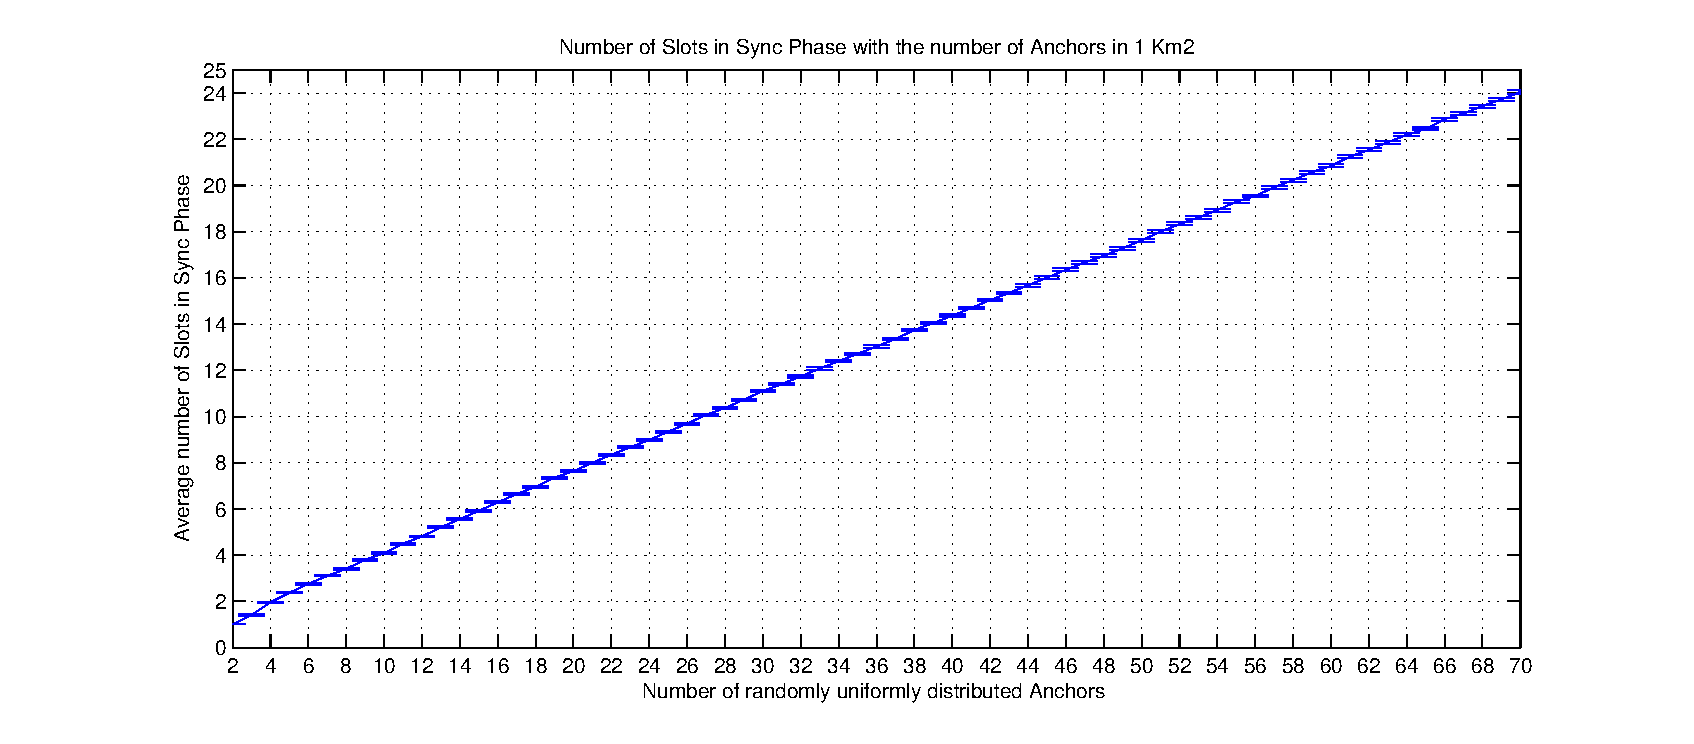
\includegraphics[width=0.8\textwidth]{numberOfSlotsWithTheAnchorDensity.eps}
 \end{center}
 \caption{Slot Number for a variable \acp{AN} density}
 \label{fig:numberOfSlotsWithTheAnchorDensity}
\end{figure}

\textbf{Figure \ref{fig:numberOfSlotsWithTheAnchorDensity}} is the result of simulating a 1 $Km^2$ playground with a number of \acp{AN} going from 
2 to 70, as the playground is fixed and only the number of nodes increase, it could be said that \acp{AN} density increases. When \acp{AN} density 
increases, and as \acp{AN} range stays constant, the number of neighbors for each \ac{AN} increases also. This makes the number of slots grow together
with the number of \acp{AN}, as it can be seen in the figure.

\begin{figure}[ht]
 \begin{center}
  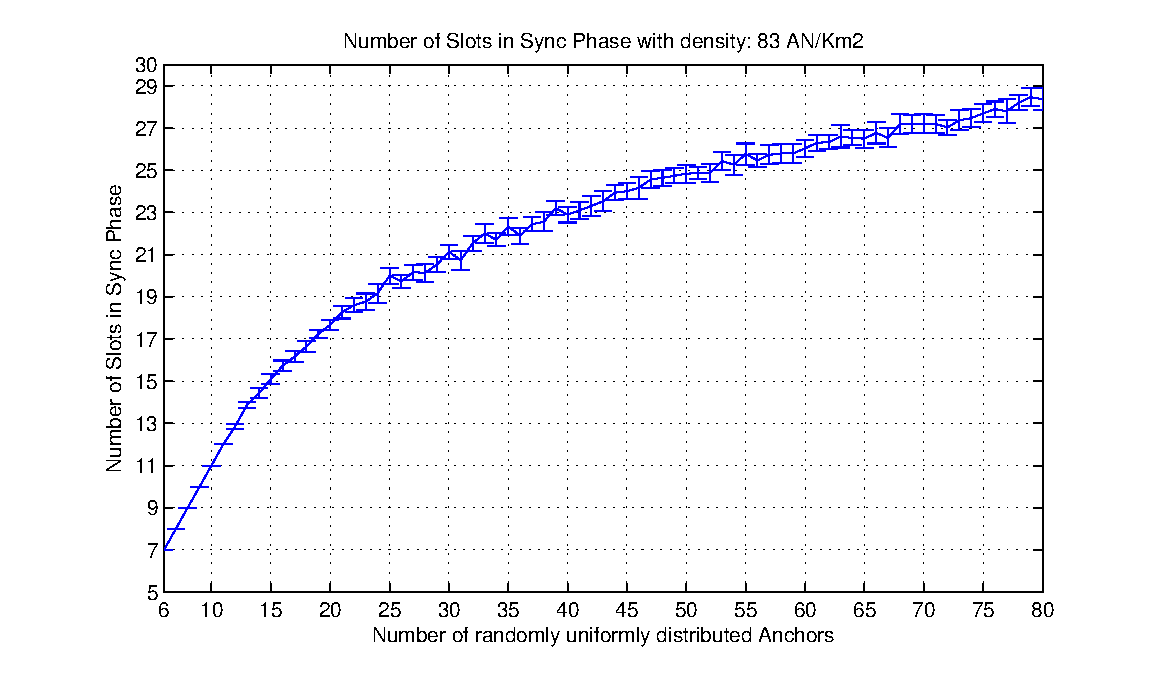
\includegraphics[width=0.8\textwidth]{numberOfSlotsWithTheSameDensity.eps}
 \end{center}
 \caption{Slot Number for a fixed \acp{AN} density}
 \label{fig:numberOfSlotsWithTheSameDensity}
\end{figure}

In this case, \textbf{Figure \ref{fig:numberOfSlotsWithTheSameDensity}} is obtained simulating 6 to 80 nodes with a minimum separation between them of 
80 meters. Playground is calculated dynamically with this parameters to have always a 83 $\acp{AN}/Km^2$ density. As \acp{AN} density remains constant,
the number of neighbors an \ac{AN} has also does. This means the re-usability of the slots will grow with the number of nodes. The re-usability can be
observed in the figure, as when the number of \acp{AN} grow, the number of slots does not grow linearly like in Figure 
\ref{fig:numberOfSlotsWithTheAnchorDensity}.

\subsubsection{Checking the best inter packet random time}

In this scenario, each \ac{AN} sends as many packets as it can during the Sync Phase time defined by the slots. First, Computer calculates the number of
slots and multiplies it by \textit{syncPacketsPerSyncPhase} (in this case 3) to obtain the Sync Phase time. This simulation will be done for different
number of \acp{AN} (already told) and different maximum random times between transmissions from 1 to 30 ms. After repeating each case 100 times,
\textbf{Figure \ref{fig:randomTimeCheckingTheBestInterpacketRandomTime}} is obtained.

\begin{figure}[ht]
 \begin{center}
  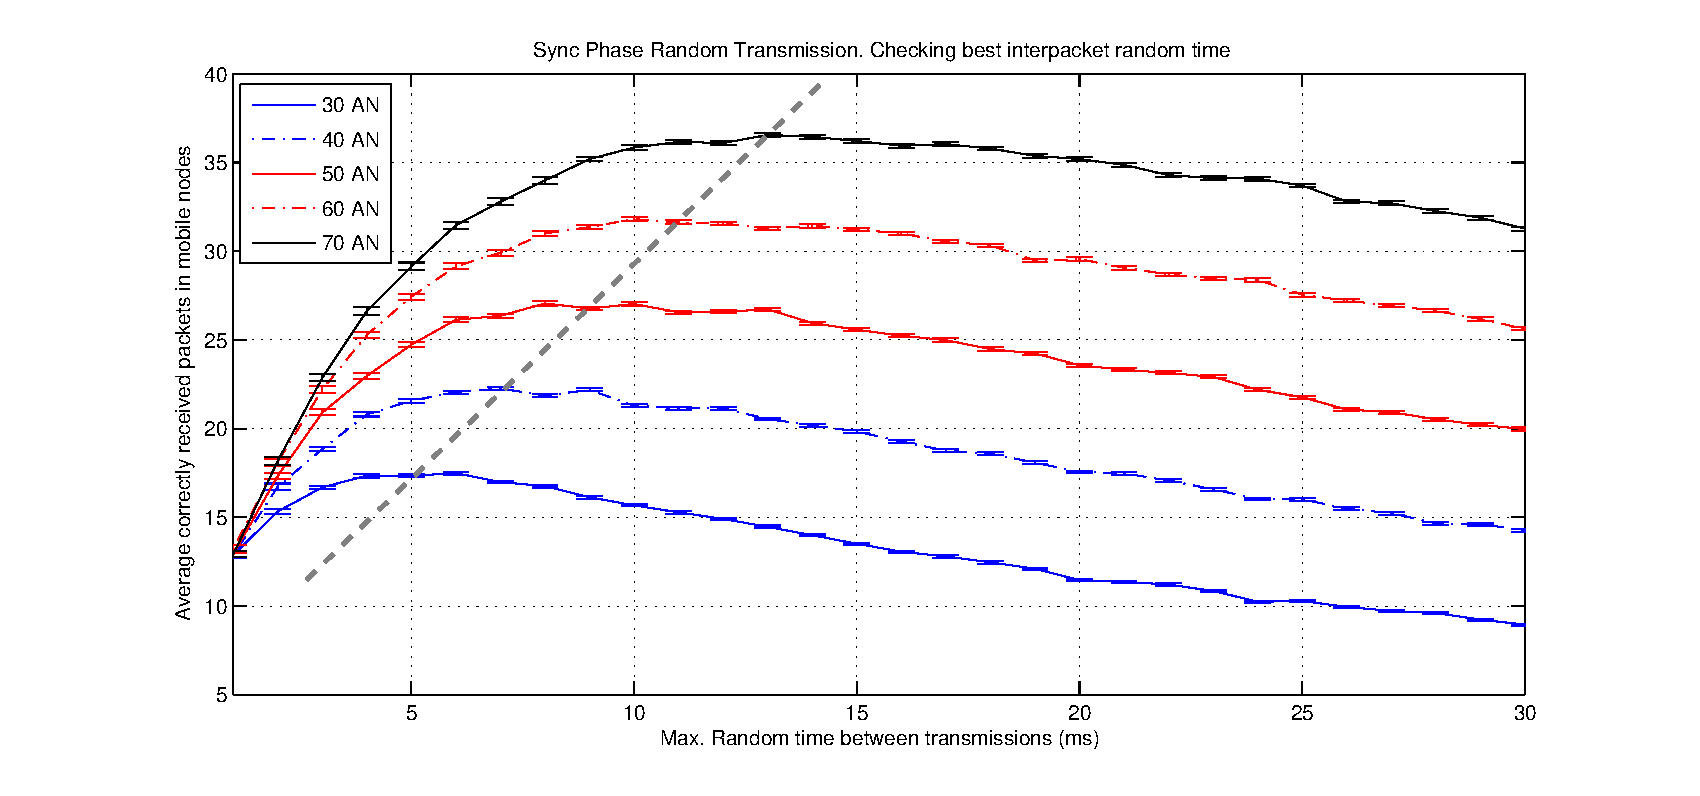
\includegraphics[width=1\textwidth]{randomTimeCheckingTheBestInterpacketRandomTime.eps}
 \end{center}
 \caption{Checking the best time between random transmissions}
 \label{fig:randomTimeCheckingTheBestInterpacketRandomTime}
\end{figure}

In this figure, it can be seen how when the time between transmissions is small, the number of delivered packets is also small. This is due to the 
collisions. When the time between transmissions grows, so does the correctly received packets until it reaches a maximum where it goes down again.
The ground for this is that the bigger the time between transmissions is, the less the number of packets that fit in the fixed Sync Phase time. When in 
Figure \ref{fig:receivedPacketsAndLastPacketArrival} there was no time limit, it could be seen how the received packets number did only grow.

From Figure \ref{fig:randomTimeCheckingTheBestInterpacketRandomTime}, it can also be seen that the more \acp{AN} there are, the more received packets and
the later the maximum comes. This maximum comes later because as the number of \acp{AN} is bigger, there are also more collisions, being its effect in the 
number of delivered packets bigger compared with the time between transmissions. And as the number of slots is bigger (hence the Sync Phase time), the 
time between transmissions influence will come later.

The gray discontinuous line was drawn following the maximum points for every curve. This line gives us the optimum waiting time between transmissions to 
be set for any number of \acp{AN}. Taking a smaller value generates more collisions and a bigger value makes the number of delivered packets smaller due
to the lack of time in the phase.

\subsubsection{Checking the best number of sent packets per \ac{AN}}

In this scenario, each \ac{AN} sends a maximum number of packets from 3 to 16 during the Sync Phase time defined by the slots. First, Computer calculates 
the number of slots and multiplies it by \textit{syncPacketsPerSyncPhase} (in this case 3) to obtain the Sync Phase time. This simulation will be done 
for different number of \acp{AN} (already told) where the previous optimal maximum random times between transmissions will be taken (see Table
\ref{tab:optimalTransmitTimes}). After repeating each case 100 times, \textbf{Figure \ref{fig:randomTimeCheckingTheBestNumberOfSentPacketsForAnchor}} 
is obtained.

\begin{table}
 \begin{center}
  \begin{tabular}{|l|c|}
   %\noalign{\vspace*{0.5cm}}
   \hline
   30 \acp{AN} & 5 ms \\
   \hline
   40 \acp{AN} & 7 ms \\
   \hline
   50 \acp{AN} & 9 ms \\
   \hline
   60 \acp{AN} & 11 ms \\
   \hline
   70 \acp{AN} & 13 ms \\
   \hline
  \end{tabular}
  \caption{Optimal maximal random times between \ac{AN} transmissions}
  \label{tab:optimalTransmitTimes}
 \end{center}
\end{table}

\begin{figure}[ht]
 \begin{center}
  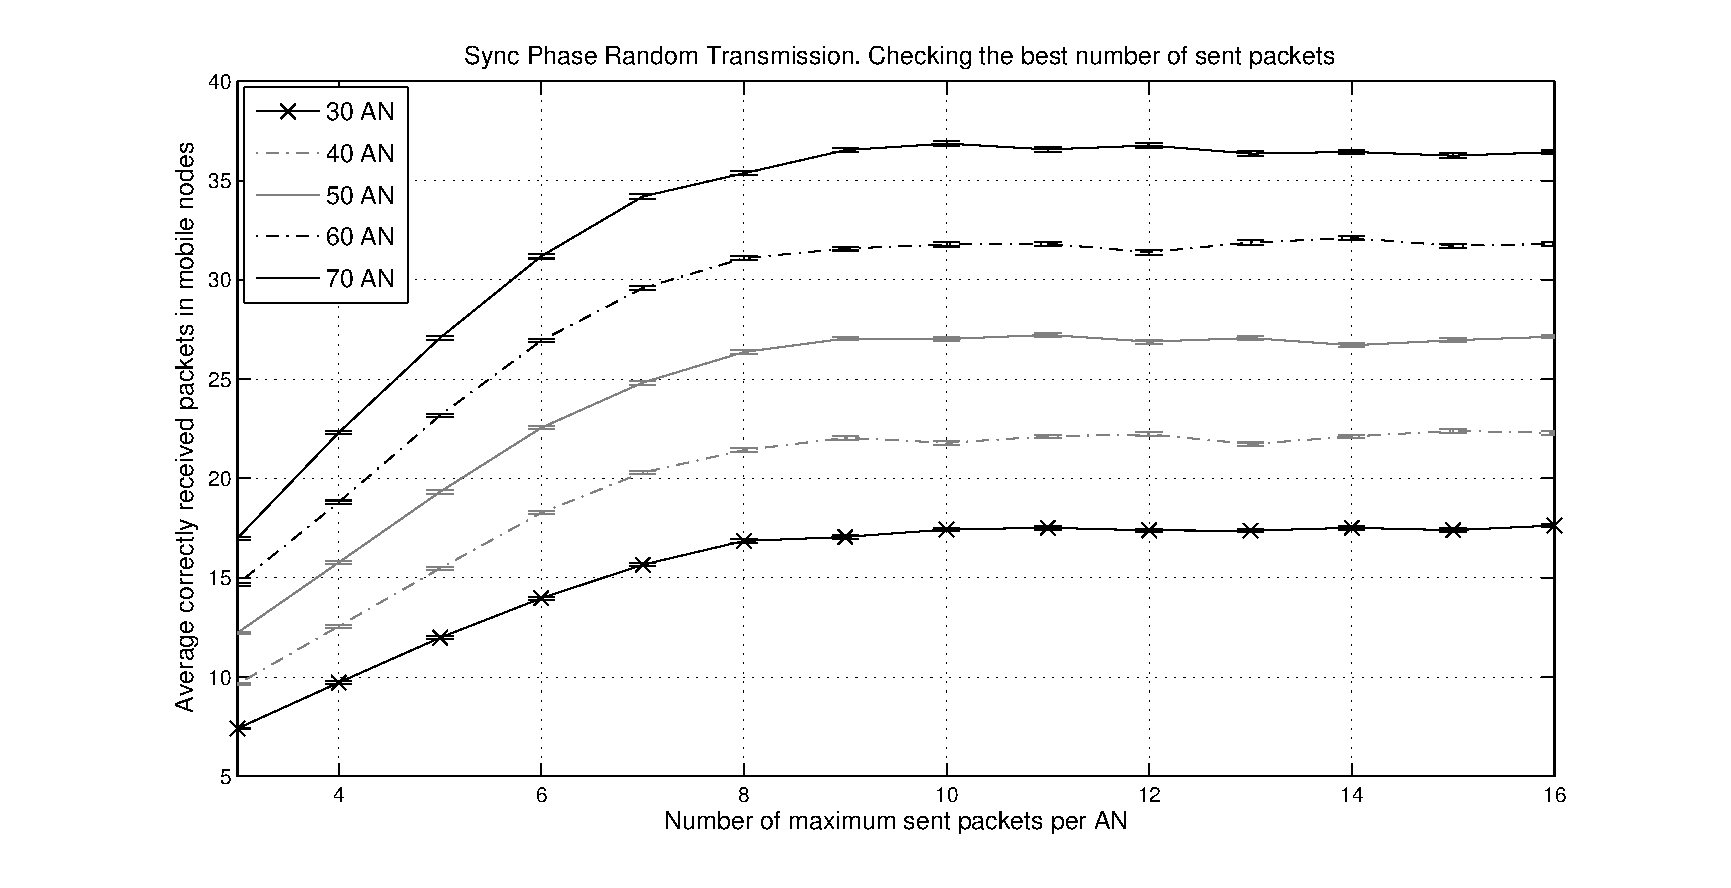
\includegraphics[width=1\textwidth]{randomTimeCheckingTheBestNumberOfSentPacketsForAnchor.eps}
 \end{center}
 \caption{Checking the best number of sent packets per \ac{AN}}
 \label{fig:randomTimeCheckingTheBestNumberOfSentPacketsForAnchor}
\end{figure}

It can be clearly seen in the figure, how the average number of received packets in the \acp{MN} increases until it reaches a maximum (approximately
with 10 sent packets). This is so because in the fixed Sync Phase time, there is no time for more packets to arrive. Ten is hence defined as the 
maximum number of packets to be sent. The reason to this limit is that when an \ac{AN} has already reached this maximum sent packets number per Sync Phase, 
it will stop sending more, leaving the channel more free for the rest of the \acp{AN} to transmit.

\subsubsection{Slotted vs. Best Random case comparison}

Both alternatives will be compared in a first approach checking the average number of packets received by the \acp{MN} in different situations. In 
all situations, cases with 30, 40, 50, 60 and 70 \acp{AN} will be studied. In the comparison there will be included the following situations: 
slotted case, best random transmissions case, worst random transmissions case ($T=1 ms$) and two random transmissions cases between worst and best cases
($T=3ms$ and $T=5ms$). Where T is the maximum random time between transmissions. In all cases the number of transmitted packet per \ac{AN} will be 10.

\begin{figure}[ht]
 \begin{center}
  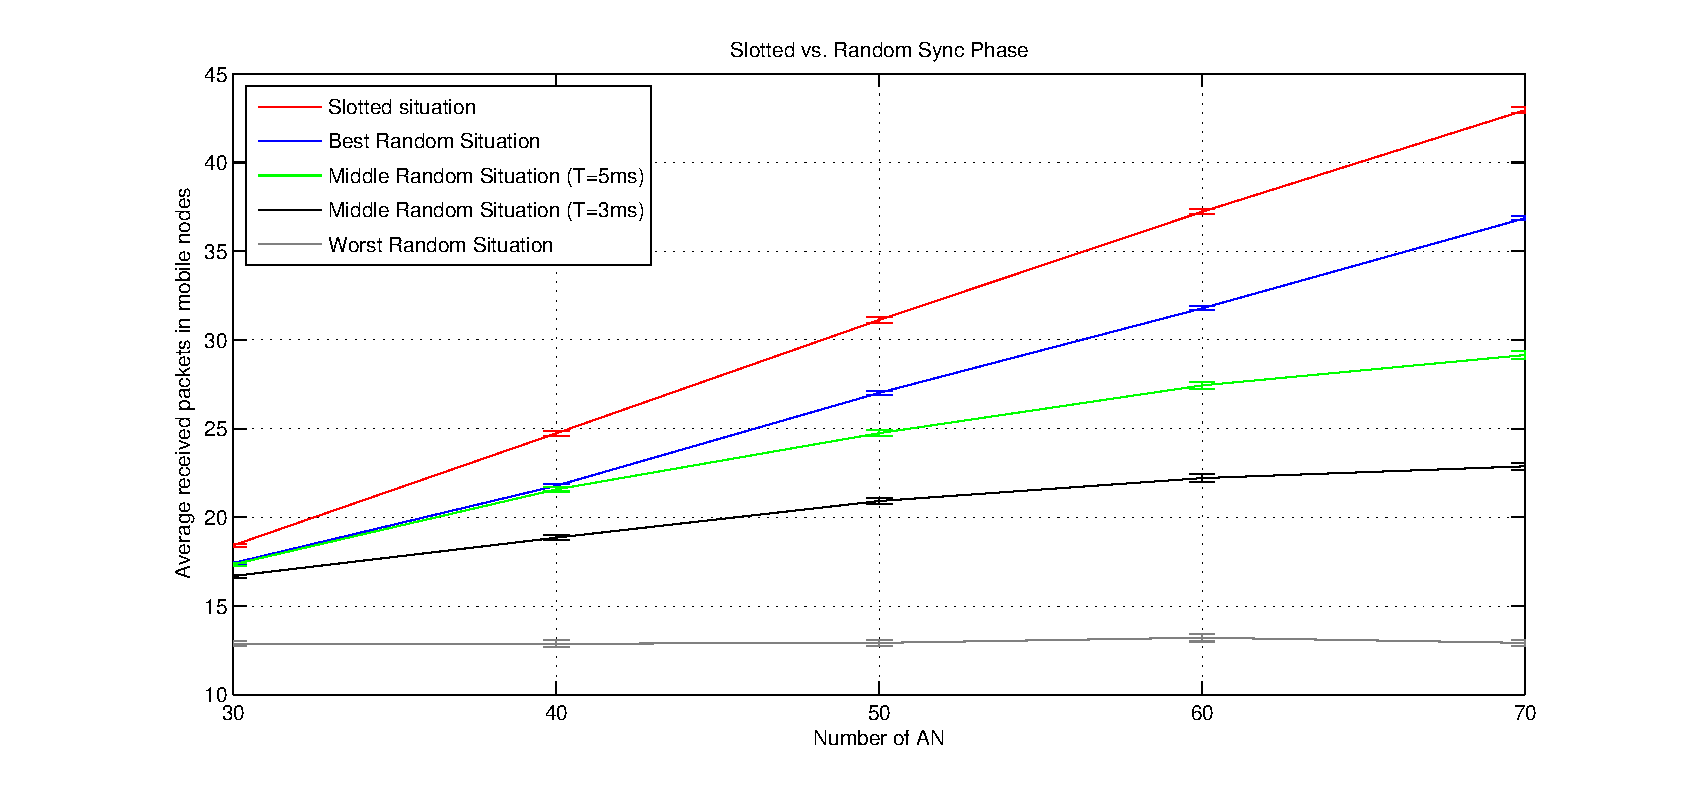
\includegraphics[width=1\textwidth]{slottedVsRandomAverageReceivedPackets.eps}
 \end{center}
 \caption{Slotted vs. Random cases comparison for number of received packets in \ac{MN}}
 \label{fig:slottedVsRandomAverageReceivedPackets}
\end{figure}

\textbf{Figure \ref{fig:slottedVsRandomAverageReceivedPackets}} shows how in all situations, in the slotted case \acp{MN} received more packets as in
any of the random cases. It can be also seen that this difference gets bigger when the number of \acp{AN} arises.

As a second comparison between the bestFrom all this, it can be obtained that slotted transmission is better than even the best case of random transmission. Slotted transmission will be hence
the one used during the Sync Phase in the complete protocol analysis. case for random transmissions and the slotted case, the number of first, second, third, fourth, \ldots, eighth
packets from an \ac{AN} received in the \ac{MN}, will be studied. Results can be seen in \textbf{Figure \ref{fig:numberOf1st2ndPacketsReceived}}.

\begin{figure}[ht]
 \begin{center}
  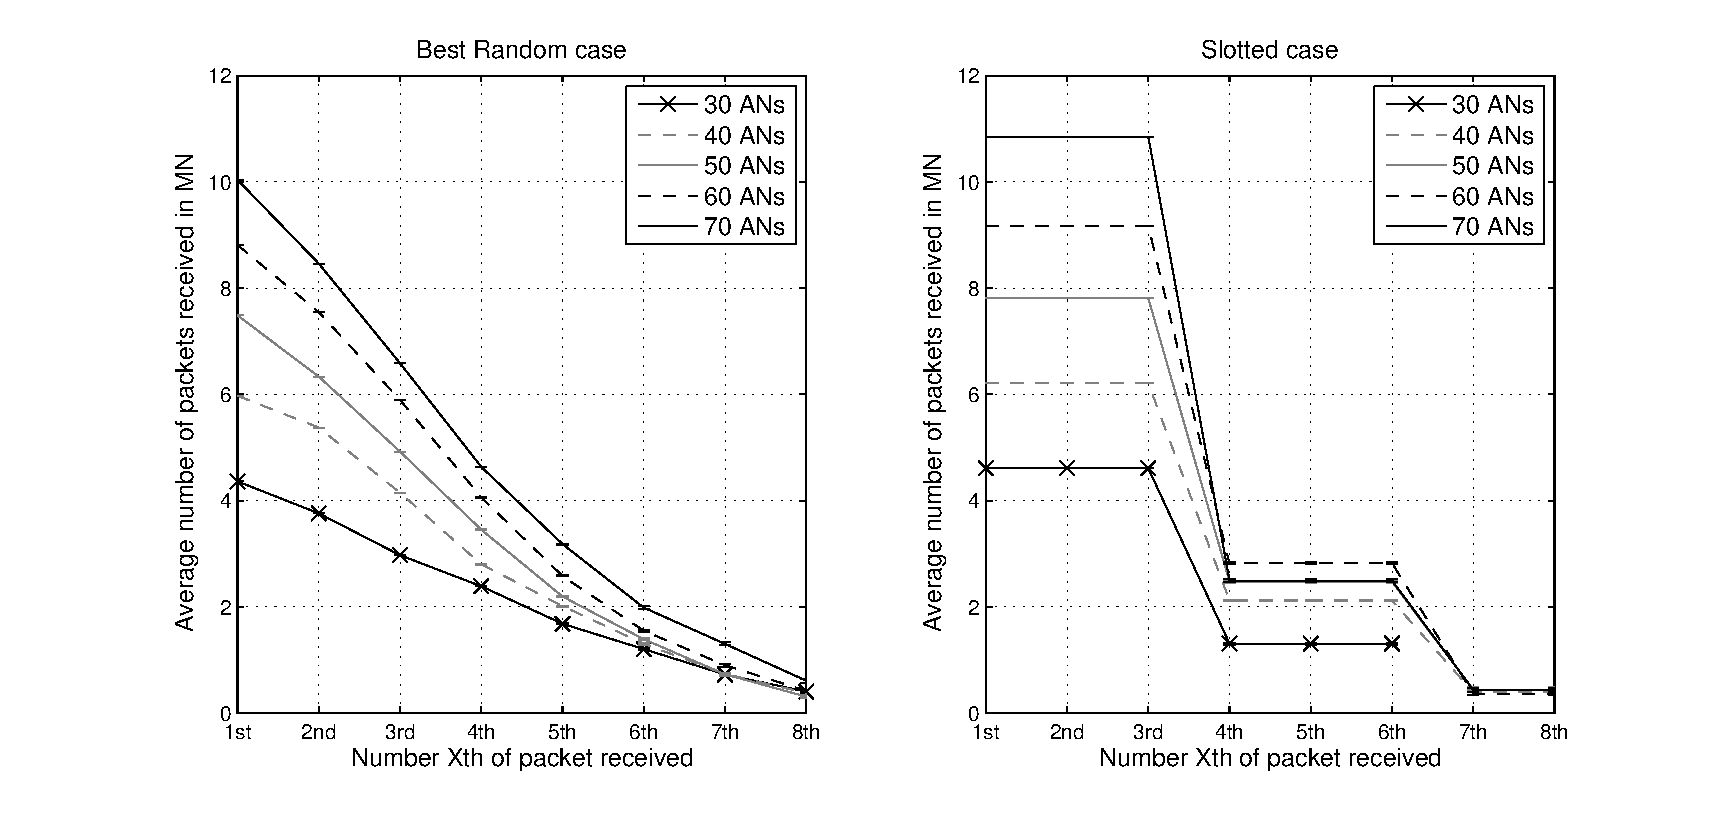
\includegraphics[width=1\textwidth]{numberOf1st2ndPacketsReceived.eps}
 \end{center}
 \caption{Number of $1^{st}$, $2^{nd}$, $3^{rd}$ \ldots, $8^{th}$ received packets in \acp{MN} from an \ac{AN}}
 \label{fig:numberOf1st2ndPacketsReceived}
\end{figure}

In both graphics can be appreciated how the more \acp{AN} there are, the more received packets in the \acp{MN}. It can be seen as well, how
for the slotted case, the number of received packets is bigger than for the random case (as it was already proved).

In the graphic on the left, it can be seen how the number of first packets received is bigger than the number of second packets. How the number of 
second packets received is bigger than the number of third packets, etc. And how this reduction occurs in a gradual way. Unlike this, in the graphic 
on the right, a stair-shaped behavior can be appreciated.

As \textit{syncPacketsPerSyncPhase} = 3, the Sync Phase will be divided into 3 identical sub phases. This means that all packets sent in one sub 
phase, will be sent in the other two. That is why the number of first, second and third packets is the same, as well as the number of fourth, fifth 
and sixth, and the number of seventh and eighth. Anytime a packet is sent more than \textit{syncPacketsPerSyncPhase} = 3 times, is due to slot re-using. 
That justifies why for example for the 30 \acp{AN} case, no seventh or eighth packets where sent, re-use here was not so big.

As a last comparison between slotted case and best random case, Packet arrival times in the \acp{MN} will be studied. Getting \textbf{Figure
\ref{fig:Lastarrivalpackettimes}} as the result to be commented. For a good understanding of this figure, X axis should be clarified. X axis has numbers
going from 1 to 11. Number from 1 to 8 represent the $1^{st}$, $2^{nd}$, $3^{rd}$ \ldots, $8^{th}$ last received packet in the \acp{MN}. Number 9 
represents the first packet arrived in the \acp{MN}. Number 10 represents the last packet arrived in the \acp{MN}. And number 11 represents the elapsed 
time between arrived packets in the \acp{MN}.

\begin{figure}[ht]
 \begin{center}
  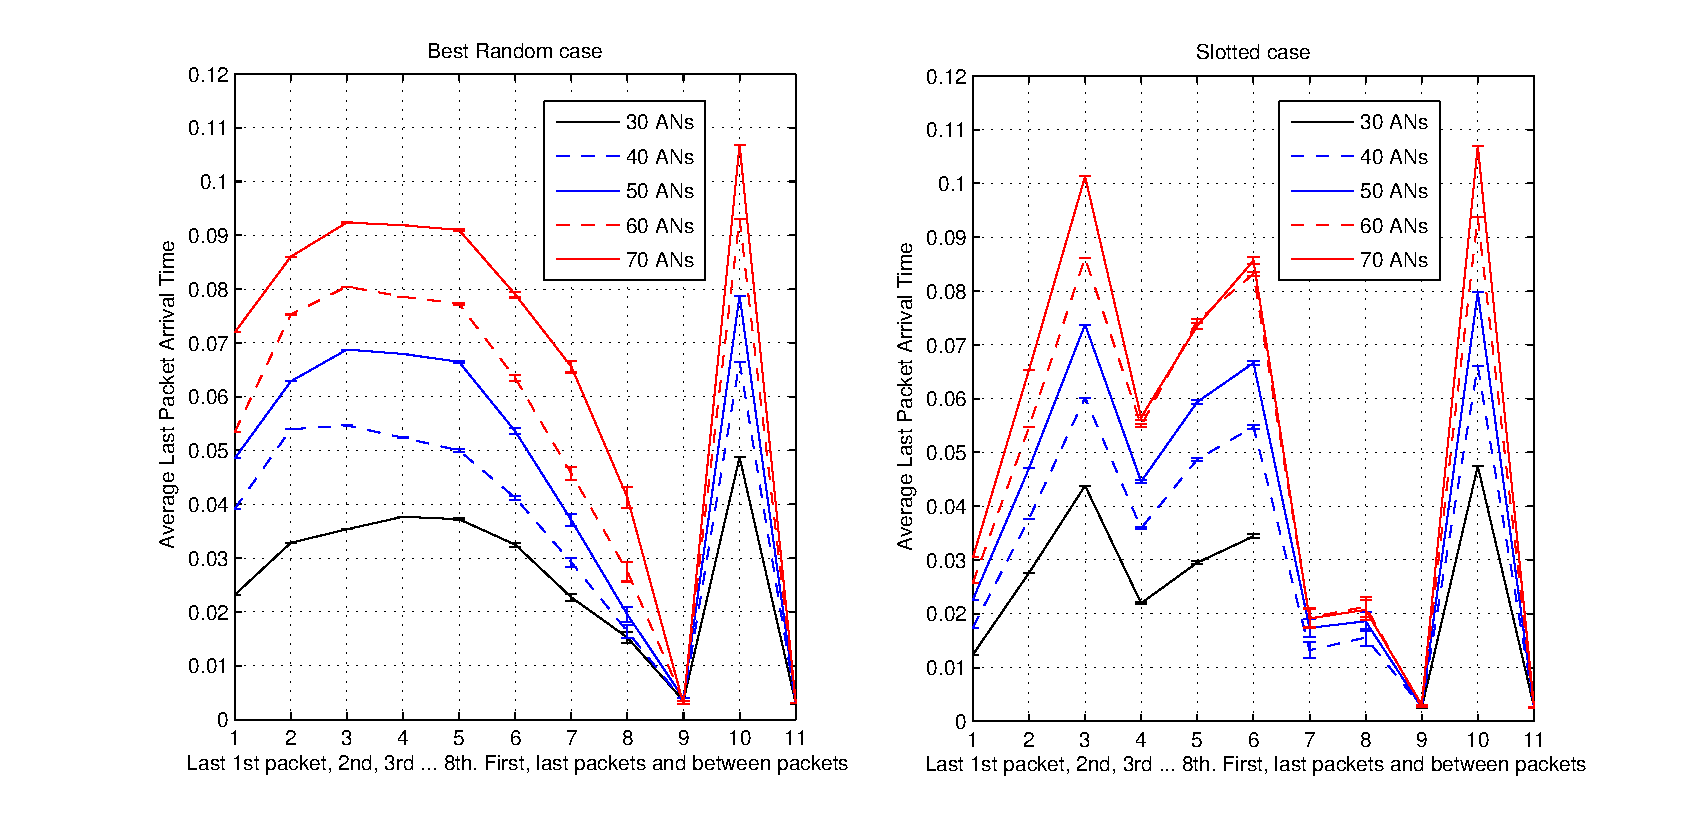
\includegraphics[width=1\textwidth]{Lastarrivalpackettimes.eps}
 \end{center}
 \caption{Different packet arrival times in the \acp{MN}}
 \label{fig:Lastarrivalpackettimes}
\end{figure}

Like for case in Figure \ref{fig:numberOf1st2ndPacketsReceived}, the more the \acp{AN} in the network, the bigger the time the \acp{MN} have to wait 
until they get the last packet.

Comparing both right and left graphics, it can be seen that the arrival times for the first ($X=9$) and last packet ($X=10$) and inter the arrival 
time ($X=11$), are very similar. This is so because this depends mainly on the duration of the Sync Phase more than on the way the packets are sent. 
Looking at the arrival time of the last packet ($X=10$), the length of the Sync Phase can be deduced. When looking to X axis values from 1 to 8, many
differences can be observed.

In the case of the graphic on the left (best random case), it can be seen that for small X values, the time of the last $X^{th}$ received packet 
grows with X. This is because all \acp{MN} receive many $1^{st}$, $2^{nd}$ or $3^{rd}$ packets, and the last of the $1^{st}$ packets should arrive 
before the last of the $2^{nd}$ and so on. But, why is it not like this until the last packet? The reason is that not many \acp{AN} are able to send
$5^{th}$, $6^{th}$, $7^{th}$ or $8^{th}$ packets being the $3^{rd}$ or $4^{th}$ the maximum packet they get to send. They are not able to send them
because the Sync Phase is limited in time, being than the $3^{rd}$ or $4^{th}$ packet sent at the end of the phase, raising thus the average arrival time
for this kind of packets.

In the slotted case graphic (on the right), the idea is the same as expressed before. The only difference is that, like in Figure 
\ref{fig:numberOf1st2ndPacketsReceived}, as \textit{syncPacketsPerSyncPhase} = 3, all behaviors are grouped. It can be seen that $1^{st}$, $2^{nd}$ and 
$3^{rd}$ last packets are together in one group. $4^{th}$, $5^{th}$ and $6^{th}$ last packets together in another group, and $7^{th}$ and $8^{th}$ in
another. Inside these groups the last $X^{th}$ arrived packet grows with X because, as the three sub phases in Sync Phase are the same, whenever a 
$4^{th}$ packet is delivered, this means that also a $5^{th}$ and $6^{th}$ packet will be.

Here it can also be observed, like in Figure \ref{fig:numberOf1st2ndPacketsReceived}, the re-usability of the slots. Seeing for example for the 
30 \acp{AN} case, that no seventh or eighth packets where sent because the re-use here was not so big.

\paragraph{Conclusion.} From all this results, it can be extracted that slotted transmission is better than even the best case of random transmission. 
Slotted transmission will be hence the one used during the Sync Phase in the complete protocol analysis.

\section{Framework simulation and analysis}

The aim of this section, is to analyze through different configurations the performance of the network for parameters like traffic or energy 
consumption among others.

The proposed scenario for this simulations is formed by 25 \acp{AN} distributed forming a grid, 60 \acp{MN} randomly and uniformly distributed in the
playground and a Computer. This scenario, with a size of 700 x 700 m, can be seen in Figure \ref{fig:finalscenario} . The \acp{AN} 
are distributed forming a grid to avoid the necessity to make a more complex routing protocol (explained in Chapter \ref{chap:protocolimplementation}: 
\nameref{chap:protocolimplementation}). Grid was also chosen because it was seen in many literature as a good standard way to study a network.

From the proposed grid, and with the help of the algorithm to assign slots (Sub-Section \ref{subsec:slottedsyncphase}: 
\nameref{subsec:slottedsyncphase}), it was obtained that 9 slots are the necessary ones to avoid Hidden Terminal Problem. This slots have the 
following distribution of \acp{AN}:

\begin{verbatim}
      Slot 0: 0, 3, 15, 18
      Slot 1: 1, 4, 16, 19
      Slot 2: 2, 17
      Slot 3: 5, 8, 20, 23
      Slot 4: 6, 9, 21, 24
      Slot 5: 7, 22
      Slot 6: 10, 13
      Slot 7: 11, 14
      Slot 8: 12
\end{verbatim}

\begin{figure}[ht]
 \begin{center}
  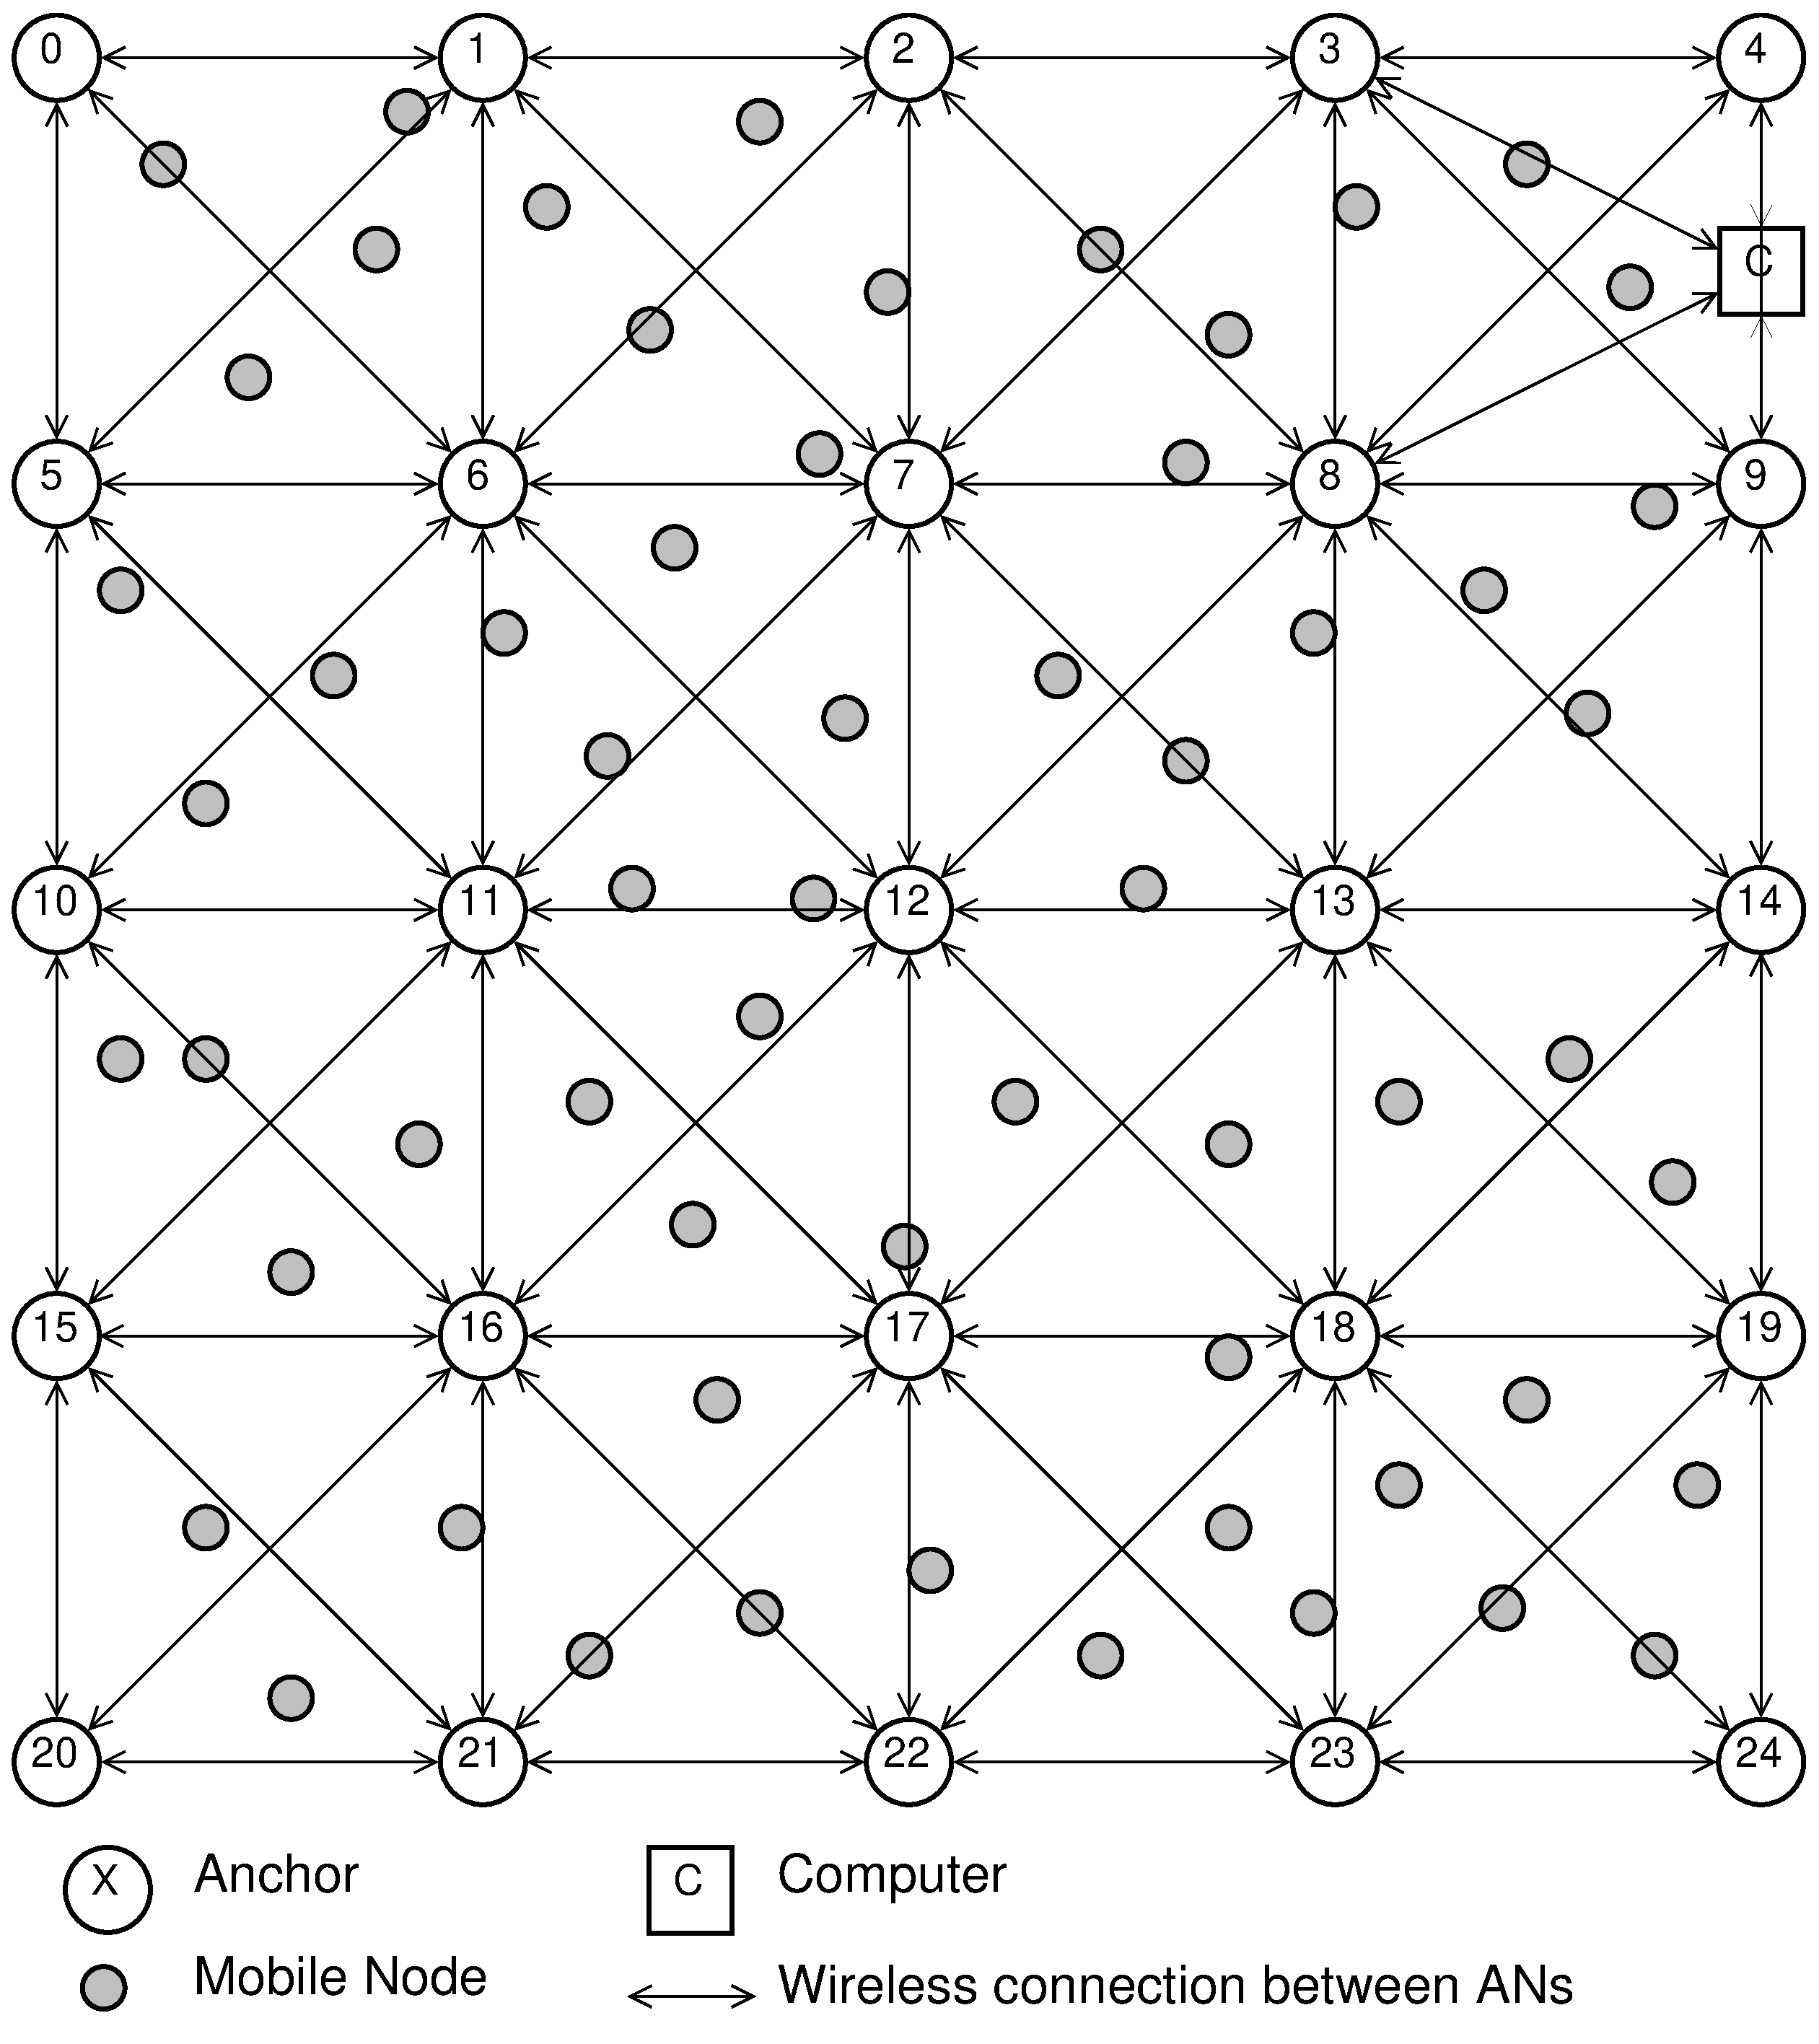
\includegraphics[width=0.5\textwidth]{finalscenario.eps}
 \end{center}
 \caption{Proposed scenario for High Configurable Protocol analysis}
 \label{fig:finalscenario}
\end{figure}

Considering that the period time is 1.5 s, the Com Sink Phases are 0.5 s each one and that there are $9\cdot3$ slots in each Sync Phase with 1.5 ms each one
of them. The following phases times are obtained:

\begin{verbatim}
    Sync Phases length:     0.0405 s
    Report Phase length:    0.2271 s
    VIP Phase length:       0.1514 s
    Com Sink Phases length: 0.5000 s
\end{verbatim}

To force different simulation situations and to be able to check the different \acp{MN} modes, ten configurations are going to be proposed. This 
configurations could be changed just modifying some parameters (explained in Section \ref{sec:ProtocolDescription}: \nameref{sec:ProtocolDescription}). 
Each one of this configurations is going to be simulated during 120 s (80 periods), and repeated 100 times to be able to compensate the dispersion 
generated by the generated random numbers. All graphics in this section will have on X axis this configurations.

The configurations are divided into two groups:

\begin{itemize}
 \item \textbf{Non distributed. }Groups the first five configurations, which are going to be the ones loading the network the most. All of this
configurations are going to have the following parameters in common:
\begin{verbatim}
 activePhases = 1
 inactivePhases = 0
 offsetPhases = 0
 offsetSyncPhases = 0
 reportPhases = 4 
 askFrequency = 2
 offsetReportPhases = 0
 NumberOfBroadcasts = 5
\end{verbatim}
As all the offsets are set to zero, all \acp{MN} will start their functionality at the beginning of the first period and all at the same
time. This is the reason why this group is called ``non distributed''. As it can be observed, inactive periods are set to 0, this way, all \acp{MN} will 
work every period, loading the network all the time. As \textit{reportPhases} = 4, \acp{MN} Mode 2 and 3 will report only 1 out 4 periods, loading even
more the network during this periods. Note also that the number of broadcast per \ac{MN} Mode 3 and 4 are five. This five configurations are taken as
 worst case and will be used to have a worst limit to compare with the other ones.

From this group, and attending to the number of \acp{MN} of each Mode (see Figure \ref{fig:ProtocolPhases}) this 5 configurations are proposed:
\begin{itemize}
 \item[-] \textbf{Config 1}: 15 \acp{MN} Mode 1, 15 \acp{MN} Mode 2, 15 \acp{MN} Mode 3 and 15 \acp{MN} Mode 4.
 \item[-] \textbf{Config 2}: 6 \acp{MN} Mode 1, 6 \acp{MN} Mode 2, 15 \acp{MN} Mode 3 and 33 \acp{MN} Mode 4.
 \item[-] \textbf{Config 3}: 6 \acp{MN} Mode 1, 6 \acp{MN} Mode 2, 33 \acp{MN} Mode 3 and 15 \acp{MN} Mode 4.
 \item[-] \textbf{Config 4}: 33 \acp{MN} Mode 1, 15 \acp{MN} Mode 2, 6 \acp{MN} Mode 3 and 6 \acp{MN} Mode 4.
 \item[-] \textbf{Config 5}: 15 \acp{MN} Mode 1, 33 \acp{MN} Mode 2, 6 \acp{MN} Mode 3 and 6 \acp{MN} Mode 4.
\end{itemize}
 \item \textbf{Distributed. }Groups the last five configurations, which are going to be the ones loading the network the less. All this
configurations are going to have the following parameters in common:
\begin{verbatim}
 activePhases = 2
 inactivePhases = 4
 offsetSyncPhases = 1
 reportPhases = 12
 askFrequency = 2
 NumberOfBroadcasts = 3
\end{verbatim}
This time, it can be seen that both \textit{offsetPhases} and \textit{offsetReportPhases} are not common parameters, this is because they are going to be
used to distribute all the \acp{MN} in the time in a way that $1/3$ of the \acp{MN} will start in period 0, another $1/3$ will start in period 2 and the 
rest $1/3$ will start in period 4. As \textit{activePhases} + \textit{inactivePhases} = 6, \acp{MN} will be perfectly distributed to load the network as 
low as possible. Due to the different kinds of \acp{MN}, the distribution in time will be done equally for every kind of \ac{MN}.

As \textit{reportPhases} = 12, \acp{MN} Mode 2 and 3 will report only 1 out 12 periods, that means they will almost not load the network. Note also that 
the number of broadcast per \ac{MN} Mode 3 and 4 is three instead of five. This five configurations are a possible normal way of loading the network, and
they will be compared with the worst case to see if performance gets improved.

From this group, and attending to the number of \acp{MN} of each Mode (see Figure \ref{fig:ProtocolPhases}) this 5 configurations are proposed:
\begin{itemize}
 \item[-] \textbf{Config 6}: 15 \acp{MN} Mode 1, 15 \acp{MN} Mode 2, 15 \acp{MN} Mode 3 and 15 \acp{MN} Mode 4.
 \item[-] \textbf{Config 7}: 6 \acp{MN} Mode 1, 6 \acp{MN} Mode 2, 15 \acp{MN} Mode 3 and 33 \acp{MN} Mode 4.
 \item[-] \textbf{Config 8}: 6 \acp{MN} Mode 1, 6 \acp{MN} Mode 2, 33 \acp{MN} Mode 3 and 15 \acp{MN} Mode 4.
 \item[-] \textbf{Config 9}: 33 \acp{MN} Mode 1, 15 \acp{MN} Mode 2, 6 \acp{MN} Mode 3 and 6 \acp{MN} Mode 4.
 \item[-] \textbf{Config 10}: 15 \acp{MN} Mode 1, 33 \acp{MN} Mode 2, 6 \acp{MN} Mode 3 and 6 \acp{MN} Mode 4.
\end{itemize}
Each of this configurations divide the number of \acp{MN} from each mode by 3, assigning the first third \textit{offsetPhases} = 0 and 
\textit{offsetReportPhases} = 2, the second third \textit{offsetPhases} = 2 and \textit{offsetReportPhases} = 4 and the third third
\textit{offsetPhases} = 4 and \textit{offsetReportPhases} = 6. This way all nodes will be equally distributed. That is why this group is called
``Distributed''. 
\end{itemize}

From all the previous times and parameters, it can be obtained that in configurations 1 to 5 the \acp{MN} send the following number of packets during
every simulation depending on the Mode they work:
\begin{itemize}
 \item Each \ac{MN} in Mode 1, sends 80 reports and 0 broadcasts (one report in each period).
 \item Each \ac{MN} in Mode 2, sends 30 reports and 0 broadcasts (20 ask reports + 10 request reports).
 \item Each \ac{MN} in Mode 3, sends 30 reports and 300 broadcasts (during 20 report phases, does not send broadcasts).
 \item Each \ac{MN} in Mode 4, sends 80 reports and 400 broadcasts (one report and five broadcasts in each period).
\end{itemize}
The same could be obtained for configurations 6 to 10:
\begin{itemize}
 \item Each \ac{MN} in Mode 1, sends 22 reports and 0 broadcasts (13 reports + 6 extra reports + 3 requests).
 \item Each \ac{MN} in Mode 2, sends 9 reports and 0 broadcasts (6 extra reports + 3 requests).
 \item Each \ac{MN} in Mode 3, sends 9 reports and 78 broadcasts (three broadcasts each active period).
 \item Each \ac{MN} in Mode 4, sends 22 reports and 78 broadcasts (13 + 6 + 3 reports, three broadcasts each active period).
\end{itemize}

As a first orientation result and trying to depict what the following analysis will show, in Table \ref{tab:simulationtimes}, it could be seen the times 
the computer took to simulate each one of the configurations. This gives a first idea of the different network loads, meaning more load more simulation
time.

\begin{table}
 \begin{center}
  \begin{tabular}{|l|c|}
   %\noalign{\vspace*{0.5cm}}
   \hline
   Configuration 1 & 7 hours 53 min \\
   \hline
   Configuration 2 & 8 hours 57 min \\
   \hline
   Configuration 3 & 8 hours 35 min \\
   \hline
   Configuration 4 & 6 hours 20 min \\
   \hline
   Configuration 5 & 5 hours 55 min \\
   \hline
   Configuration 6 & 5 hours 14 min \\
   \hline
   Configuration 7 & 6 hours 26 min \\
   \hline
   Configuration 8 & 6 hours 12 min \\
   \hline
   Configuration 9 & 3 hours 16 min \\
   \hline
   Configuration 10 & 2 hours 59 min \\
   \hline
  \end{tabular}
  \caption{Simulation times depending on Configuration}
  \label{tab:simulationtimes}
 \end{center}
\end{table}

\subsection{Traffic in the network}

To give an idea of the traffic in the network for the different configurations, \acp{AN} must be studied. All reports or broadcasts generated by the
\acp{MN} are later on retransmitted to the coordinator (in all cases a centralized schema was used). \acp{AN} are the ones in charge of distributing this
information as well as routing the information coming from and to the computer. This is why Com Sink phases are going to be the ones loaded
the most and hence their study the most interesting to be studied.

\begin{figure}[ht]
 \begin{center}
  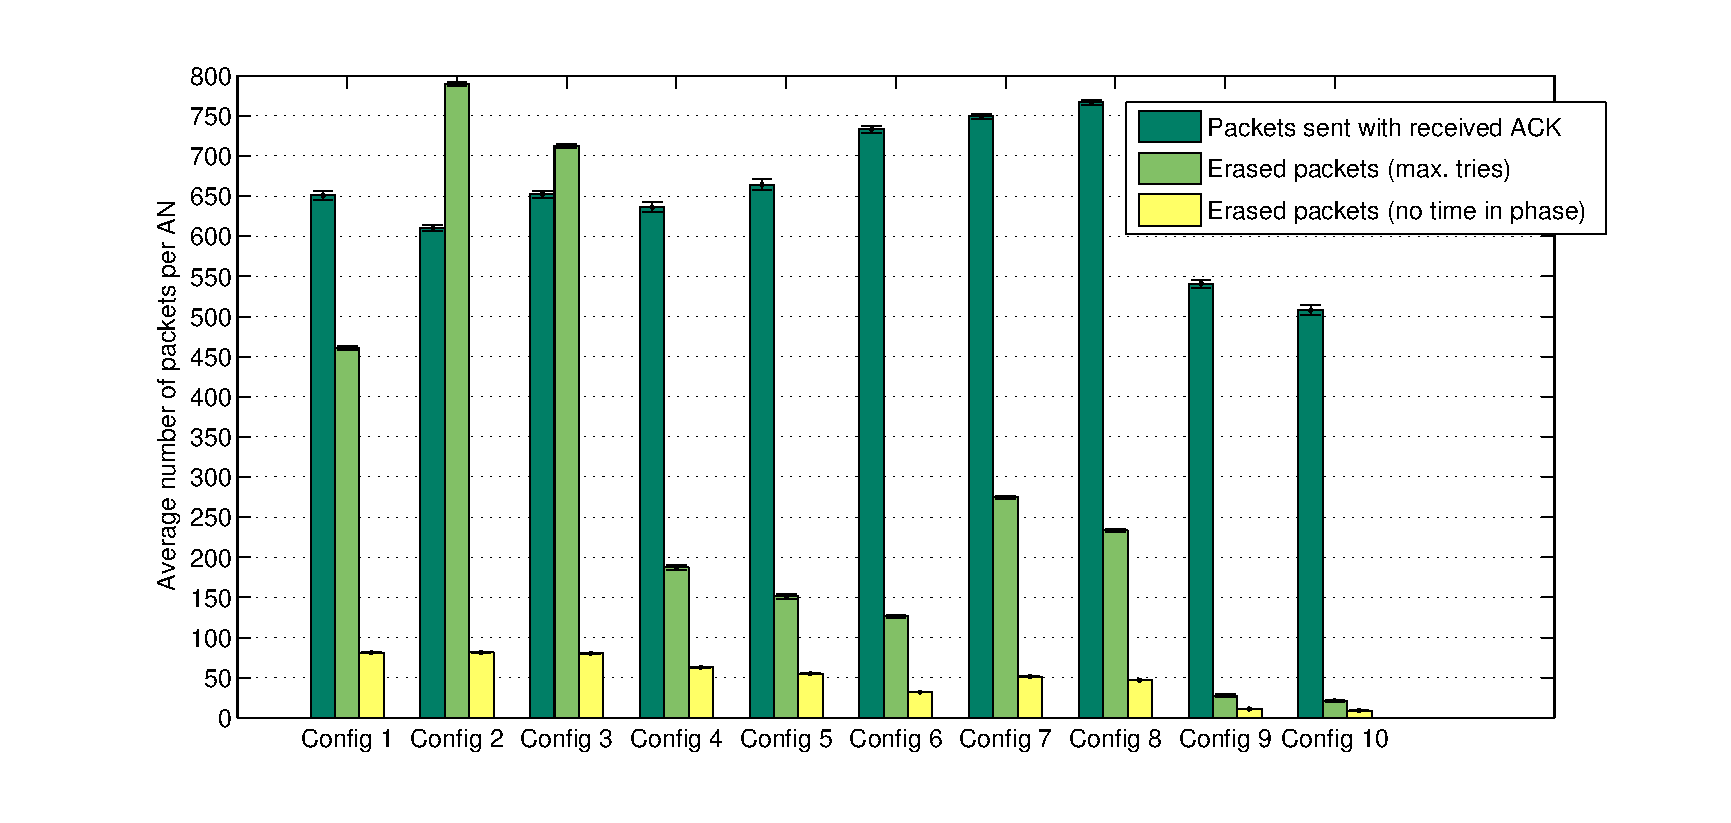
\includegraphics[width=1\textwidth]{packetsSentErasedNoTimeAN.eps}
 \end{center}
 \caption{Traffic statistics for the \acp{AN}}
 \label{fig:packetsSentErasedNoTimeAN}
\end{figure}

In \textbf{Figure \ref{fig:packetsSentErasedNoTimeAN}}. Erased packet due to maximum number of retransmissions are more in non-distributed 
configurations than in the distributed ones. This is because in non-distributed ones, all \acp{MN} transmit in every period, generating much more traffic
that in distributed ones. This makes the \acp{AN} traffic in Com Sink phases bigger than the one the channel can absorb, eliminating thus many packets 
due to the high number of collisions they had.

When a \ac{MN} sends a broadcast, unlike for reports, this packet reaches more than one \ac{AN} generating X times the traffic of a report (X = number of \acp{AN}
who received the broadcast). This is the reason why in the figure it can be observed that for configurations 2 and 3 or 7 and 8 where the number of 
\acp{MN} who broadcast are increased, the number of erased packets due to maximum number of retransmissions is increased respecting configurations
1, 4 and 5 or 6, 9 and 10.

In the case of configurations 1, 2 and 3, there are many erased packets, some times even more than correctly sent packets. All this deletions, motivate
that for configurations 6, 7 and 8, as the number of collisions is smaller, the number of successfully delivered packets is bigger even when for 
distributed configurations, the total number of sent packets by the \acp{MN} is smaller.

Erased packets due to a lack of time in the phase, are the erased packets when the end of Com Sink phases is approaching (10 ms of guard time is left
before the end of the phase). When a change of phase comes, all scheduled packets to be sent, must be deleted or postponed, otherwise they will be 
transmitted during the next Sync Phase, provoking non desired collisions.

As for the deleted packets before, erased packets are more in the non-distributed case. In configurations 1, 2 and 3 can be seen how this value
reaches a maximum, being the same in the three cases. If this is compared with the distributed case, as this value does not saturate, the logic behavior 
can be seen, where for configuration 1, the deleted packets are less than for the configurations where there are more \acp{MN} in Modes 3 and 4 and hence 
more broadcasts. This saturation value is reached because there are so many collisions, that the \acp{AN} do not receive more packets to be routed.
When the guard time comes, the \acp{AN} only have to send the own generated packets scheduled to be sent some time before, and the ones to be routed 
which managed to be delivered with all the network saturation.

\subsection{Transmission efficiency in \acp{MN}}

In this sub-section an idea of the efficiency of a \ac{MN}'s transmission is given. This will be done by analyzing the average number of \ac{CSMA/CA}
Backoffs and their average time before a transmission gets to be done. The number of retries done due to a lack of \ac{ACK}, will be also analyzed.

\begin{figure}[ht]
 \begin{center}
  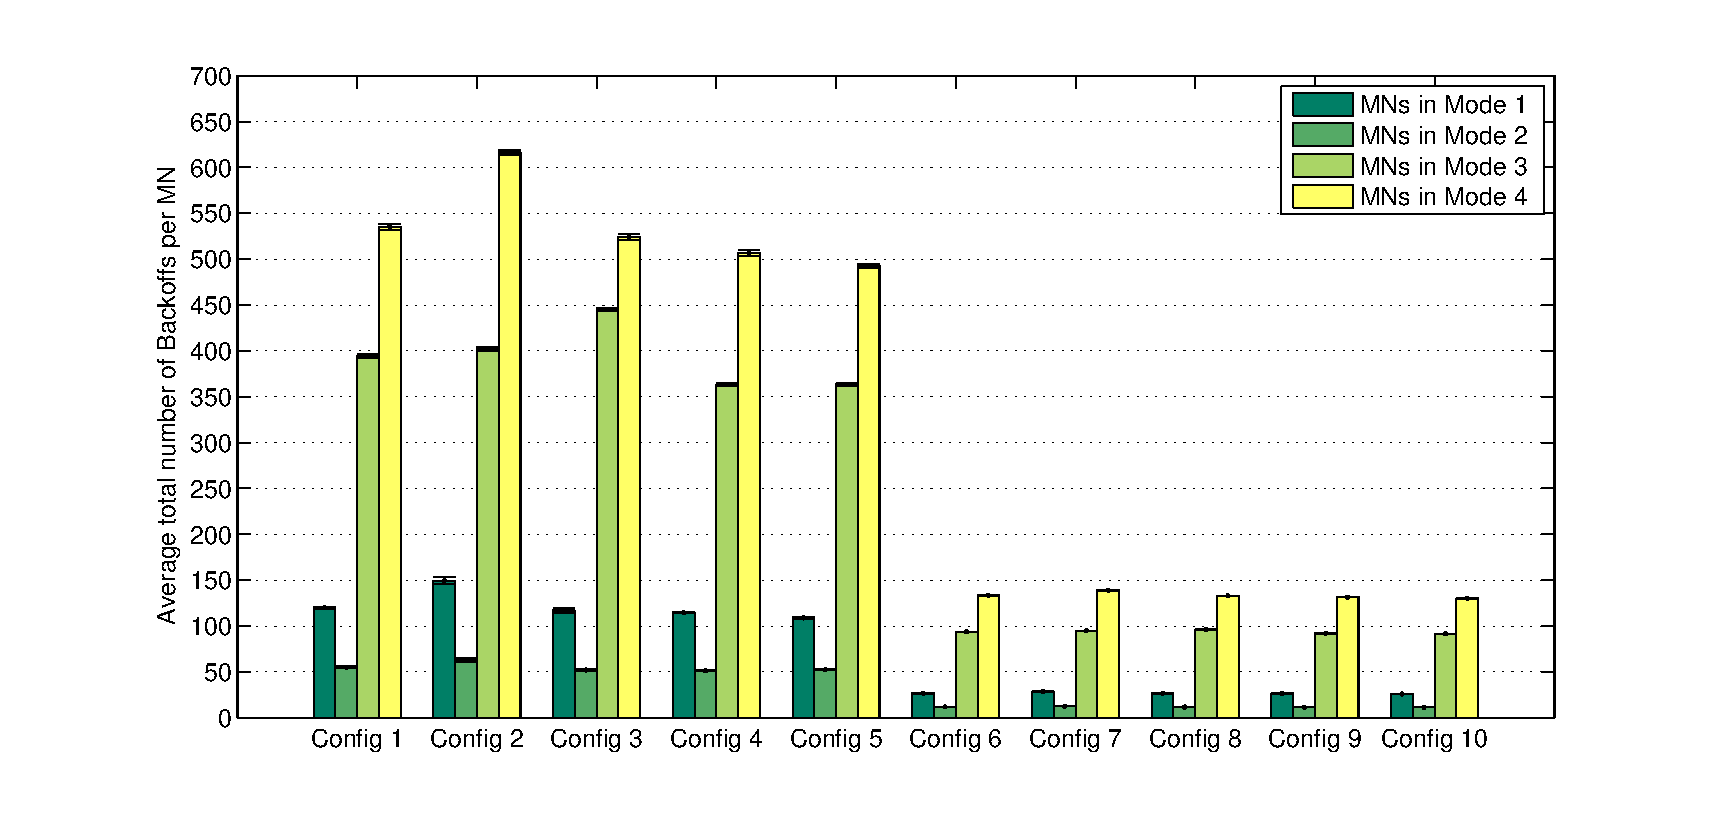
\includegraphics[width=1\textwidth]{BackoffNumberInMN.eps}
 \end{center}
 \caption{Average Backoff number for different modes and configurations}
 \label{fig:BackoffNumberInMN}
\end{figure}

In \textbf{Figure \ref{fig:BackoffNumberInMN}} can be easily seen how for the configurations 1 to 5, when the network is more loaded, the number of 
average Backoffs is bigger than for the normal case in configurations 6 to 10. This is due to the total sent packets number.

It is in general seen that \acp{MN} in modes 3 and 4, which send broadcasts, have a bigger number of Backoffs than \acp{MN} in modes 1 and 2. The same 
happens between \acp{MN} in mode 1, which have more than \acp{MN} in mode 2. As each packet needs at least one Backoff independently of the type of 
packet, this difference is caused by the total number of sent packets by each \ac{MN} in each mode. This difference is bigger for the configurations 1 
to 5 because, as the number of packets sent to channel is bigger, the \acp{MN} find more often the channel busy and thus they need at least another Backoff
period.

In configurations 6 to 10 can be seen that all values are very similar independently of the configuration. As all packets to be transmitted have at least
one Backoff period, this constant values are showing the minimum number of Backoffs. As this configurations almost do not load the network, this values 
depend basically on the number of packets to be sent.

In configuration 2 for example, it can be observed how as the number of \acp{MN} in mode 4 was arisen, the Report Phase will be more loaded, and average
Backoff periods needed by \acp{MN} in modes 1, 2 and 4 will grow in comparison with configuration 1 (equilibrated configuration), specially for \acp{MN} in
mode 4. \acp{MN} in mode 3 do not get affected so much because they have their own phase to transmit.

In configurations 4 and 5, when the number of only transmitting reports \acp{MN} is arisen, the average number of Backoff periods goes down in general,
this is because reports do not charge the network like broadcasts do.

It is interesting also to see that for configuration 3, where \acp{MN} in mode 3 are predominant, almost only \acp{MN} in mode 3 are affected. This is so
because they have their own phase (\ac{VIP} Phase) to transmit, and their transmissions do not affect the other modes.

\begin{figure}[ht]
 \begin{center}
  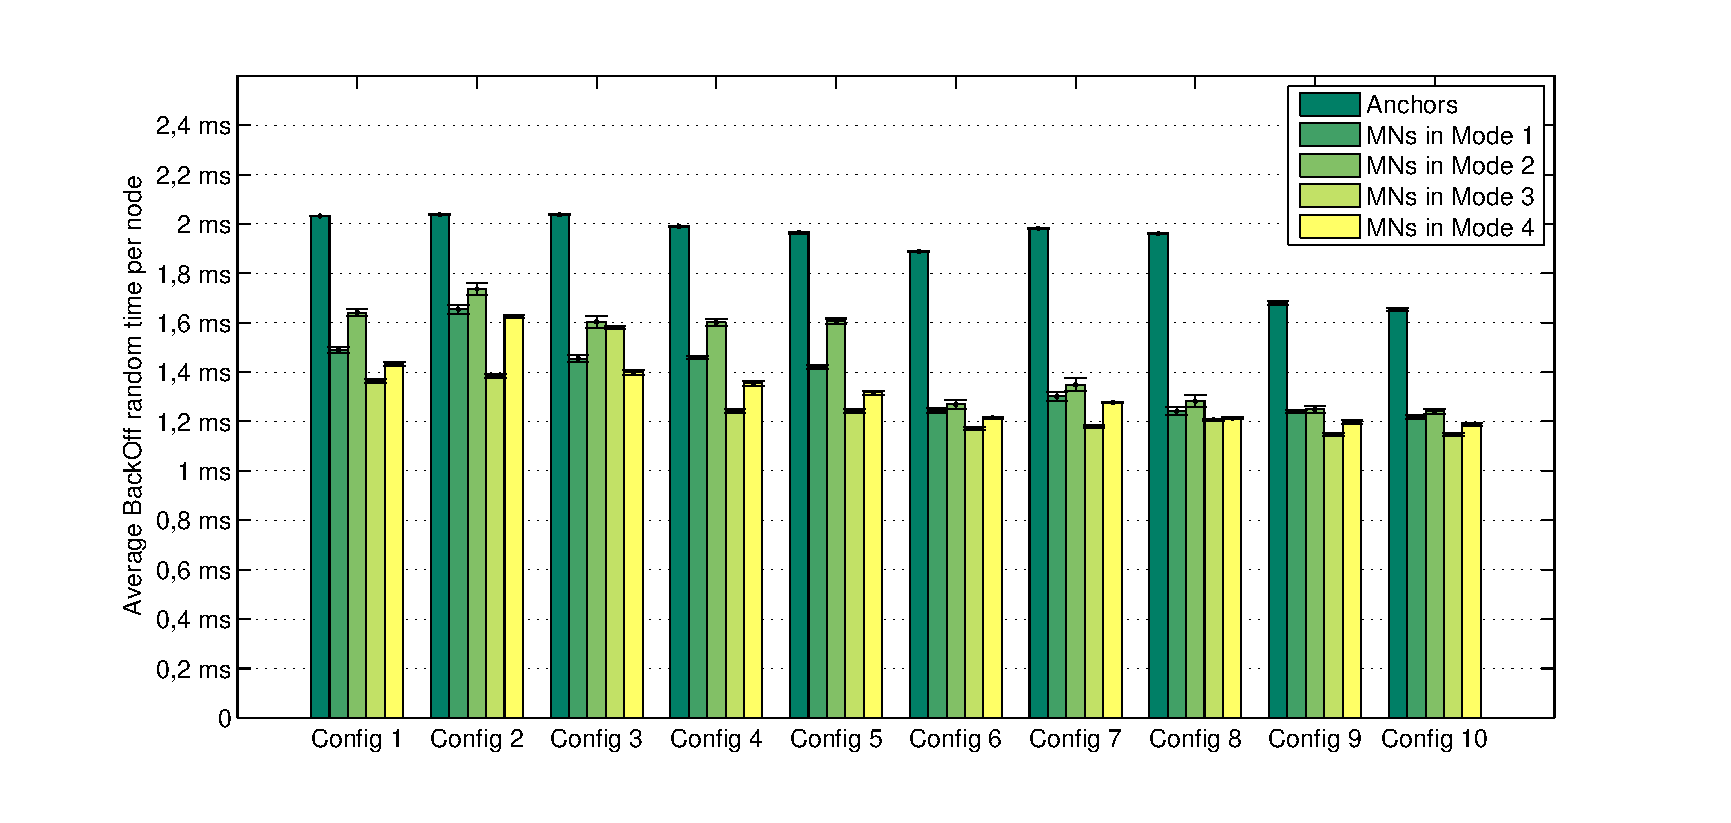
\includegraphics[width=1\textwidth]{averageBackoffTimeANandMN.eps}
 \end{center}
 \caption{Average Backoff times for different nodes and configurations}
 \label{fig:averageBackoffTimeANandMN}
\end{figure}

For a good analysis of \textbf{Figure \ref{fig:averageBackoffTimeANandMN}}, it needs to be observed that according to (\ref{mat:backoffexpression}),
the first Backoff time in average is 1.12 ms.
\begin{equation}
  rand(0;  2^3-1)\cdot aUnitBackoffPeriod = rand(0; 2^3-1)\cdot 320\mu s\ \cite{IEEE802.15.4-2006}
  \label{mat:backoffexpression}
\end{equation}
With this data in mind, it can be seen in the figure that excepting for the \acp{AN}, where (as it was already said in previous sub-section) the 
number of deletions and thus retransmissions is high, all average Backoff times are not much bigger that this minimum average value. That shows that for
all configurations, even from 1 to 5 where average Backoff time is a little bit bigger, the number of Backoffs due to channel 
busy is not that high and thus the average Backoff time. The data from this figure, together with the one from Figure \ref{fig:BackoffNumberInMN} give
also an idea of the idle listening necessary for each mode to be able to transmit a packet.

From the figure can also be extracted that in configuration 2, as the network load grows, also does the average Backoff time for \acp{MN} in modes 1, 2 
and 4. \acp{MN} in mode 3 do not see their average Backoff time increased because, like it was already said, they transmit in their own phase. For this
reason can be also seen that in configuration 3, only average Backoff time for \acp{MN} in mode 3 gets considerably increased.

Configurations 4 and 5 show how decreasing the number of broadcasts in Report Phase (less \acp{MN} in mode 4), as the number of packets in the channel
gets reduced, the average Backoff time for all modes gets also reduced. This is because whenever a \ac{MN} wants to transmit a report, it is easier to 
find the channel free.

Last but not least, there is an strange detail in the figure. Why if \acp{MN} in mode 2 are the ones sending the less packets to the network, is their 
average Backoff time the biggest in all configurations? This happens because the way the network is configured, all extra report periods, match up in time
with other active periods, in configurations 1 to 5 all periods are active for all \acp{MN} and in configurations 6 to 10 all periods are active for 
some \ac{MN} (they are distributed in time). This means that, as \acp{MN} in mode 2, transmit their packets only in extra report periods, they are going to 
find always a more loaded network and thus its average Backoff time will be bigger. The other \acp{MN} in modes 1, 3 and 4 are finding also extra report 
periods loaded and are getting high Backoff time values, but, as they transmit also in calmer periods, their average Backoff time will be reduced.

\begin{figure}[ht]
 \begin{center}
  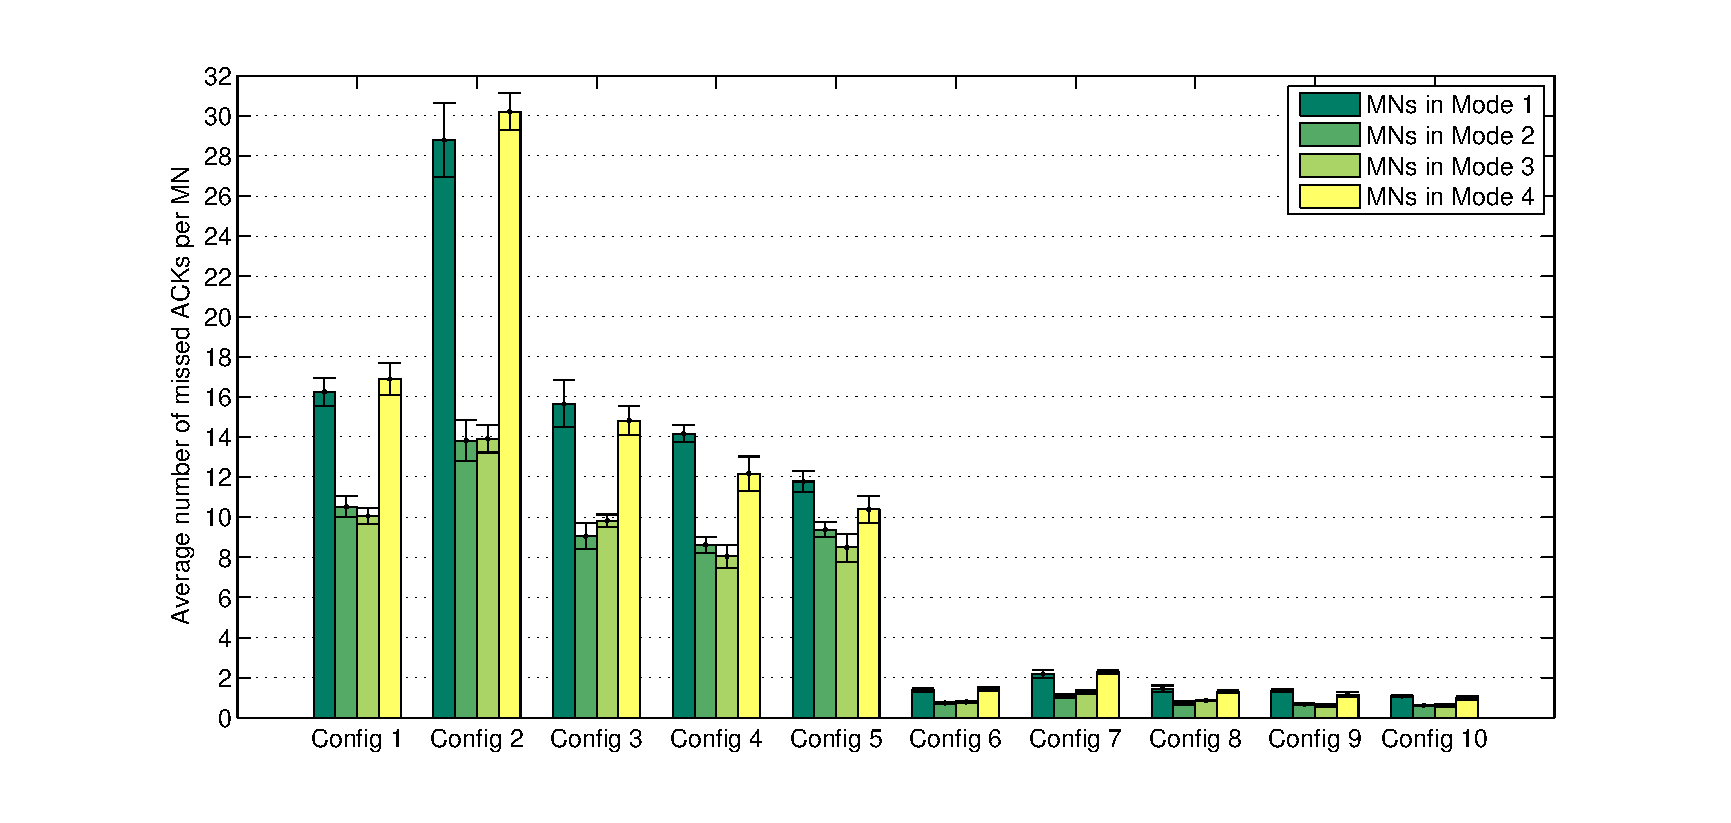
\includegraphics[width=1\textwidth]{nbMissedACKMN.eps}
 \end{center}
 \caption{Average number of report retransmissions due to the lack of ACK}
 \label{fig:nbMissedACKMN}
\end{figure}

Reports are the only packets sent by \acp{MN} where an \ac{ACK} is answered to confirm the correct packet delivery. Reports are just sent during the
Report Phase and the lack of \ac{ACK} clearly means a collision. That is why \textbf{Figure \ref{fig:nbMissedACKMN}} shows how loaded the Report Phase is
for the different configurations and how the different \acp{MN} modes get affected. As in previous figures the influence of network load was not easy to
see, in this figure it can be easily seen that for configurations 1 to 5 the number of collions is much bigger than for configurations 6 to 10.

As the lack of \ac{ACK} affects only the reports, it can be also seen how \acp{MN} in modes 1 and 4 and \acp{MN} in modes 2 and 3 get in all cases similar
values as they send almost the same number of reports.

As in configuration 2, there is a bigger number of broadcasts loading the Report Phase with much more traffic, the number of retransmissions due to 
the lack of \ac{ACK} gets much bigger.

\paragraph{Conclusion.} Number of Backoffs together with the number of retransmitted packets due to the lack of ACK, show us that \acp{MN} transmissions 
are quite efficient for this configurations, at least compared with \acp{AN} transmissions. From this results can directly be extracted that, while 
Report and VIP Phase times are good enough, the Com Sink phases times should be bigger for some of the configurations.

\subsection{Energy consumption in \acp{MN}}

As it was already said during this work, all \acp{MN} have different working states: sleep all, sleep but $\mu C$ working, idle, transmission and 
reception. Each of this states have a different energy consumption (Table \ref{tab:NodeEnergyConsumption}), and transitions between states take 
different times (Table \ref{tab:NodeTiming}). During the simulation, all \acp{MN} changed their states as explained in Section 
\ref{sec:frameworkdevelopment}: \nameref{sec:frameworkdevelopment}. Times in different state and in all possible transitions between states were stored
during 120 s. This times multiplied by the energy consumed for each case and added together, result in \textbf{Figure \ref{fig:energyConsumptionPerMN}}.

\begin{figure}[ht]
 \begin{center}
  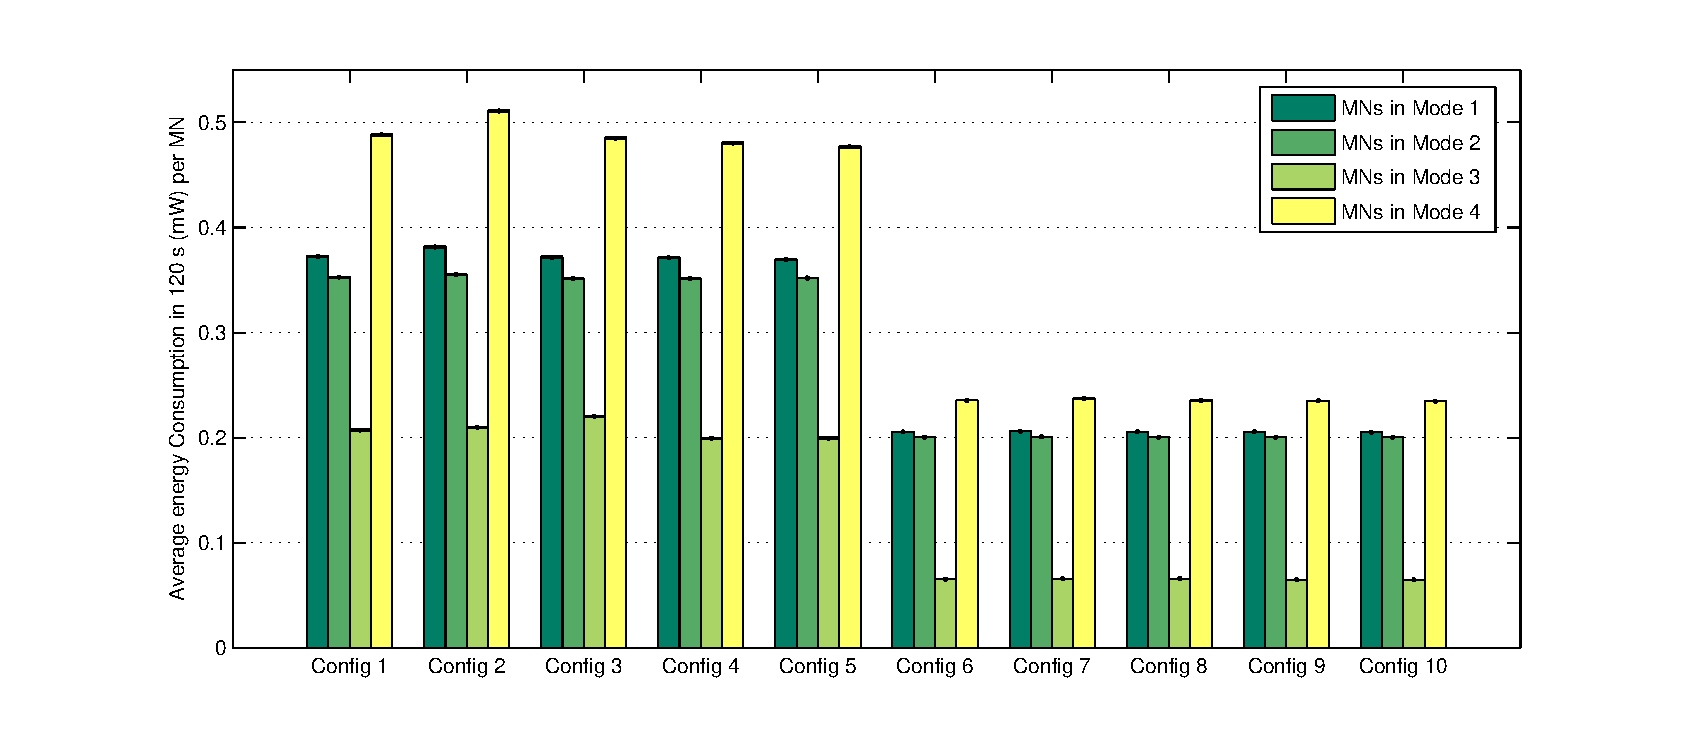
\includegraphics[width=1\textwidth]{energyConsumptionPerMN.eps}
 \end{center}
 \caption{Average energy consumed by any \ac{MN} in 120 s (mW)}
 \label{fig:energyConsumptionPerMN}
\end{figure}

Figure shows how for configurations with the same parameters (configurations 1 to 5 and 6 to 10), the consumed energy values stay approximately
constant independently of network charge. This independence, means that \acp{MN} consume most of the energy when listening during Sync Phases and 
when transmitting, but not in retransmissions due collisions. This good performance of \acp{MN} during Report and \ac{VIP} phases was already seen
in previous sub-section and it is also confirmed here. 

In configuration 3, a light growth in energy can be appreciated for \acp{MN} in mode 3. This is caused by the increment of broadcasts number to share the 
\ac{VIP} Phase. Anyway, this increment is not that big. This shows that even this mode, with a shorter in time \ac{VIP} Phase, is not very much affected
by collisions. In configuration 8, this effect is even not appreciable because instead of 5 broadcasts per \ac{MN} only 3 are sent, and also because
\acp{MN} are distributed in time, being found transmitting at the same period only $1/3$ of the \acp{MN} in mode 3.

In configuration 2, a light growth in energy for \acp{MN} in mode 4 can be also appreciated. The reason is exactly the same as for \acp{MN} in mode 3.

Another important aspect extracted from the figure is that although \acp{MN} in mode 1 transmit more reports that \acp{MN} in mode 2, their energy
consumptions are almost the same. This means that for \acp{MN} in modes 1 and 2, which do not transmit broadcasts, the biggest part of the consumed energy,
comes from listening to the Sync Phases.

A last reflexion involves \acp{MN} in mode 1 and 4. Their behavior is very similar, finding as only difference that \acp{MN} in mode 4 apart from 
listening to Sync Phases and transmitting reports, transmit also broadcasts. This way it can be noted that the difference in energy consumed for both
modes, represents the energy consumed transmitting the broadcasts. To assert this affirmation, it can be seen that for configurations 1 to 5, where
5 broadcasts per \ac{MN} in mode 4 are sent, the energy consumption difference between \acp{MN} in mode 1 and in mode 4 is bigger than for configurations
6 to 10 where the number of broadcasts per \ac{MN} in mode 4 is just 3.

